\documentclass{article}

% NeurIPS 2026 submission
\usepackage[preprint]{neurips_2026}

\usepackage[utf8]{inputenc} % allow utf-8 input
\usepackage[T1]{fontenc}    % use 8-bit T1 fonts
\usepackage{hyperref}       % hyperlinks
\usepackage{url}            % simple URL typesetting
\usepackage{booktabs}       % professional-quality tables
\usepackage{amsfonts}       % blackboard math symbols
\usepackage{amsmath}
\usepackage{amssymb}
\usepackage{amsthm}         % theorem environments
\newtheorem{assumption}{Assumption}
\newtheorem{proposition}{Proposition}
\newtheorem{corollary}{Corollary}
\newtheorem{remark}{Remark}
\usepackage{nicefrac}       % compact symbols for 1/2, etc.
\usepackage{microtype}      % microtypography
\usepackage{xcolor}         % colors
\usepackage{graphicx}       % to include figures
\usepackage{subcaption}     % for subfigures
\usepackage{algorithm}
\usepackage{algorithmic}
\usepackage{multirow}
\usepackage{colortbl}

\title{Latent Altruism: Steering Cooperative Intent\\in Large Language Models via Activation Engineering}

\author{%
  Trung Kiet Huynh\thanks{Co-first author.}\thanks{University of Science (HCMUS), VNU-HCM, Vietnam} \\
  \texttt{23122039@student.hcmus.edu.vn}
  \And
  Duy Minh Dao Sy\footnotemark[1]\footnotemark[2] \\
  \texttt{23122041@student.hcmus.edu.vn}
  \AND
  Phu Hoa Pham\footnotemark[2] \\
  \texttt{23122030@student.hcmus.edu.vn}
  \And
  Chi Nguyen Tran\footnotemark[2] \\
  \texttt{23122044@student.hcmus.edu.vn}
  \AND
  Phu Quy Nguyen Lam\footnotemark[2] \\
  \texttt{23122048@student.hcmus.edu.vn}
  \And
  The Anh Han\thanks{Corresponding author. School of Computing, Engineering and Digital Technologies, Teesside University, UK.} \\
  \texttt{T.Han@tees.ac.uk}
}

\begin{document}

\maketitle

\begin{abstract}
Large Language Models (LLMs) are increasingly deployed as autonomous decision-making agents in multi-agent systems. However, without explicit interventions, these models frequently default to selfish, defection-oriented strategies in game-theoretic settings---failing to achieve socially optimal outcomes. In this paper, we investigate the internal geometry of cooperative and selfish strategic intent \textbf{across five open-source LLMs spanning 7B--70B parameters and three architectural families} (Qwen, Llama, Mistral, Gemma). We propose a zero-shot, inference-time intervention using \textit{Activation Engineering}: by extracting a ``Cooperation Steering Vector'' from contrastive hidden states in the Iterated Prisoner's Dilemma, we consistently shift models from near-zero baseline cooperation to $\geq 93\%$ across all architectures. This vector generalizes zero-shot to unseen game environments (Stag Hunt, Chicken Game). Through layer-wise mechanistic analysis across all five models, we discover a universal \textbf{Strategic Bottleneck} phenomenon: peak Fisher Discriminability of cooperative vs.\ defective representations consistently occurs at $\sim$85--90\% network depth, regardless of architecture or model size. We benchmark Steering Vectors (SV) against Contrastive Activation Addition (CAA) and Representation Engineering (RepE), demonstrating that SV achieves the best cooperation--fluency tradeoff across all models. Finally, we characterize a dose-response relationship between activation steering and adversarial system prompts, deriving formal bounds on the required intervention strength. Our findings establish that cooperative intent is an \textbf{architecture-invariant} linear concept in transformer representations, providing both geometric understanding and an actionable tool for cooperative alignment.
\end{abstract}


\section{Introduction}
\label{sec:intro}

The rapid deployment of Large Language Models (LLMs) as autonomous agents in complex multi-agent environments~\citep{park2023generative, wang2023voyager} has raised fundamental questions about their strategic behavior. When these models interact with other agents---whether human or artificial---their decisions carry real consequences: negotiations, resource allocation, and collaborative problem-solving all require the capacity for cooperative behavior~\citep{duan2024gtbench}.

Game-theoretic evaluations have revealed a troubling pattern: LLMs often default to Machiavellian or strictly self-maximizing strategies, failing to achieve Pareto-optimal outcomes even in simple social dilemmas such as the Prisoner's Dilemma~\citep{brookman2023playing, fan2024can}. Traditional alignment methods---including few-shot prompting~\citep{wei2022chain}, reinforcement learning from human feedback (RLHF)~\citep{ouyang2022training}, and explicit cooperation instructions---are heavily context-dependent and prone to adversarial exploitation~\citep{perez2022red}. Moreover, fine-tuning approaches require significant compute and risk catastrophic forgetting~\citep{kirkpatrick2017overcoming}.

Recent work in \textit{Activation Engineering}~\citep{turner2023activation, zou2023representation, rimsky2023steering} has demonstrated that high-level behavioral concepts---including honesty, sycophancy, and moral reasoning---are encoded as approximately \textit{linear directions} in the latent representation spaces of neural networks. This suggests a provocative possibility: \textit{Can we identify and directly stimulate a generalized ``cooperative intent'' within an LLM, without altering its weights or degrading its linguistic capabilities?}

In this work, we present a comprehensive \textbf{cross-architecture} study on the geometry, generalizability, and limitations of cooperative intent across five open-source LLMs: Qwen2.5-32B-Instruct~\citep{qwen2025qwen25}, Llama-3.1-8B-Instruct and Llama-3.1-70B-Instruct~\citep{dubey2024llama3}, Mistral-7B-Instruct-v0.3~\citep{jiang2023mistral}, and Gemma-2-27B-it~\citep{team2024gemma2}. Our contributions are five-fold:

\begin{enumerate}
    \item \textbf{Cross-Architecture Strategic Bottleneck Discovery.} Across all five models, we discover that strategic discriminability peaks universally at $\sim$85--90\% network depth---Layer~57/65 in Qwen-32B, Layer~27/32 in Llama-8B, Layer~68/80 in Llama-70B, Layer~27/32 in Mistral-7B, and Layer~39/46 in Gemma-27B---establishing an \textit{architecture-invariant} ``strategic bottleneck'' phenomenon. This localization is consistent with the theoretical prediction that binary strategic concepts form one-dimensional directions at the network's abstract reasoning layers.

    \item \textbf{Zero-shot Cross-Game Generalization.} We demonstrate that a steering vector extracted \textit{solely} from the Prisoner's Dilemma transfers zero-shot to structurally distinct games---the Stag Hunt and Chicken Game---across all model families, providing evidence that LLMs encode a generalized, game-invariant concept of ``cooperation'' that is consistent across architectures.

    \item \textbf{Method Comparison and Dynamic Policy Steering with Capability Preservation.} We benchmark simple Steering Vectors (SV) against Contrastive Activation Addition (CAA)~\citep{rimsky2023steering} and Representation Engineering (RepE)~\citep{zou2023representation}, as well as a \emph{dynamic} steering policy that adapts the intervention strength $\alpha_t$ based on the opponent's last move (a latent Tit-for-Tat). SV consistently achieves the best cooperation--fluency tradeoff across all models.

    \item \textbf{Adversarial Dose-Response Analysis and Geometric Mitigation.} We systematically test the robustness of activation steering against four categories of adversarial system prompts and introduce an \emph{Orthogonal Concept Erasure} (OCE) mechanism. We discover a consistent dose-response relationship across models and derive formal bounds on the required $\alpha$ threshold (Proposition~\ref{prop:dose}).

    \item \textbf{Formal Theoretical Guarantees.} We provide proofs that the steering vector is Fisher-optimal under Gaussian assumptions (Proposition~\ref{prop:fisher}), derive Bayes error bounds via FDI (Corollary~\ref{cor:bayes}), and prove that OCE preserves $\geq 98.6\%$ of the cooperative signal (Proposition~\ref{prop:oce}).
\end{enumerate}


\section{Related Work}
\label{sec:related}

\paragraph{Game Theory and LLM Evaluation.}
Evaluating LLMs through classical game theory has become a standard methodology for probing social intelligence and strategic reasoning. \citet{brookman2023playing} simulated the Iterated Prisoner's Dilemma (IPD) and found that LLMs exhibit predominantly greedy behaviors unless heavily prompted. \citet{fan2024can} extended this analysis to multiple games and multiple models, revealing significant variation in cooperative tendencies across model families. \citet{duan2024gtbench} introduced GTBench, a comprehensive benchmark for evaluating LLMs across diverse game-theoretic scenarios. More recently, GT-HarmBench~\citep{cobben2026gtharmbench} provides 2,009 high-stakes scenarios grounded in canonical $2 \times 2$ game matrices, revealing that unsteered LLMs achieve socially optimal outcomes in only 62\% of cases. M3-BENCH~\citep{xie2026m3bench} complements outcome-based evaluation with process-aware diagnostics---evaluating behavioral trajectories, reasoning processes, and communication fidelity---ensuring that cooperative behavior reflects genuine strategic reasoning rather than superficial token-level compliance. Our work uses game theory not merely as an evaluation tool, but as a \textit{structured environment} for extracting and testing mechanistic interventions.

\paragraph{Activation Engineering and Representation Control.}
Instead of modifying model weights via RLHF or supervised fine-tuning, Activation Engineering adds bias vectors directly to hidden states during inference. \citet{turner2023activation} introduced Steering Vectors to alter model personas (e.g., shifting a model from ``helpful'' to ``harmful'' and vice versa). \citet{zou2023representation} formalized Representation Engineering (RepE), which uses PCA on contrastive stimulus--response pairs to extract behavioral directions. \citet{rimsky2023steering} proposed Contrastive Activation Addition (CAA), applying paired mean-difference vectors across multiple layers simultaneously. Our work extends these techniques to the multi-agent game-theoretic domain, providing structural localization and cross-game robustness benchmarks that prior work has not addressed.

\paragraph{Limits, Calibration, and Advanced Steering Methods.}
\citet{bas2025steer} systematically evaluated activation steering across 50 behavioral traits, establishing a hierarchical taxonomy of steerability: internal dispositions (personality, misalignment) are highly steerable, while external, knowledge-dependent traits (e.g., historical figure impersonation) are not. Crucially, they identified a strict \textbf{inverted-U response curve}: trait expression peaks at an optimal $\alpha$, beyond which coherence collapses monotonically as the hidden state is dragged off the language manifold. ContextFocus~\citep{anand2026contextfocus} demonstrated that systematic layer sweeps and multiplier calibration (identifying a precise optimal multiplier of $\alpha^* = 1.5$ for contextual faithfulness) are essential to operating near this optimum. Prototype-Based Dynamic Steering (PDS)~\citep{kayan2025pds} addresses the limitation of monolithic mean-difference vectors by clustering activation differences into multiple sub-directions via K-Means, enabling input-adaptive steering that maintains robustness even when the target behavior is explicitly suppressed in the prompt context.

\paragraph{Inference-Time Mechanism Design.}
Orthogonal to activation-level interventions, inference-time mechanism design approaches modify the agent's decision process through incentive shaping. Socially-Weighted Alignment (SWA)~\citep{mumcu2026swa} formalizes this by interpolating between private reward and estimated group welfare via a social alignment coefficient $\lambda$, establishing closed-form thresholds for phase transitions from congestion to optimal system operation. While SWA provides mathematical guarantees of Nash Equilibrium convergence, it requires resource-intensive iterative sampling and self-reflection loops. By contrast, our activation steering achieves comparable behavioral shifts with strictly $O(d)$ computational overhead during a single forward pass, though it lacks SWA's formal game-theoretic guarantees.

\paragraph{Mechanistic Interpretability of Strategic Behavior.}
Mechanistic interpretability seeks to reverse-engineer neural network computations into human-understandable algorithms~\citep{olah2020zoom, elhage2022toy}. Recent work has probed LLMs for internal representations of truth~\citep{li2024inference}, deception~\citep{azaria2023internal}, and social preferences. Our layer-wise localization of strategic intent complements this literature by identifying where \textit{in the architecture} cooperative vs.\ selfish strategy formation occurs, and how this differs from token-level prediction.

\paragraph{AI Safety and Adversarial Robustness.}
The vulnerability of aligned systems to adversarial inputs is a central concern in AI safety~\citep{perez2022red, wei2024jailbroken}. While most adversarial robustness work focuses on safety guardrails and harmful content generation, our ``Contextual Override'' analysis specifically targets \textit{behavioral alignment} interventions, demonstrating that activation engineering---despite its geometric elegance---faces quantitative (not absolute) limitations under hostile prompt contexts.


\section{Methodology}
\label{sec:method}

\subsection{Models and Computational Setup}

To establish cross-architecture generality, we evaluate five open-source instruction-tuned LLMs spanning three architectural families and a 10$\times$ parameter range (Table~\ref{tab:models}). All models are deployed with 4-bit quantization on NVIDIA H100 80GB GPUs via the Hugging Face \texttt{transformers} library. Hidden state extractions are performed on the \textbf{last token} of the prompt before generation begins.

\begin{table}[h]
\centering
\caption{Model configurations. The strategic layer $l^*$ is identified via layer-wise FDI sweeps (Section~\ref{sec:exp_localization}). The relative depth $l^*/L$ is remarkably consistent across architectures.}
\label{tab:models}
\small
\begin{tabular}{lcccccc}
\toprule
\textbf{Model} & \textbf{Params} & \textbf{Layers ($L$)} & \textbf{$d$} & \textbf{Quant.} & \textbf{$l^*$} & \textbf{$l^*/L$} \\
\midrule
Qwen2.5-32B-Instruct  & 32B & 65 & 5120 & AWQ 4-bit & 57 & 0.877 \\
Llama-3.1-70B-Instruct & 70B & 80 & 8192 & AWQ 4-bit & 68 & 0.850 \\
Gemma-2-27B-it         & 27B & 46 & 4608 & AWQ 4-bit & 39 & 0.848 \\
Llama-3.1-8B-Instruct  & 8B  & 32 & 4096 & NF4 4-bit & 27 & 0.844 \\
Mistral-7B-Instruct-v0.3 & 7B & 32 & 4096 & NF4 4-bit & 27 & 0.844 \\
\bottomrule
\end{tabular}
\end{table}

We use a unified experimental protocol across all models: identical game prompts, opponent strategies, $\alpha$ sweep values, and evaluation metrics. The primary quantitative results reported in the main text are from \textbf{Qwen2.5-32B-Instruct}~\citep{qwen2025qwen25} as the reference model; cross-model comparisons are reported in Section~\ref{sec:exp_crossmodel} and tabulated in supplementary materials.

\subsection{Game Environments}
\label{sec:games}

We evaluate the model across three classical non-zero-sum $2 \times 2$ games, each defining a distinct cooperation--defection tradeoff. The payoff matrices (row player payoffs) are:

\begin{table}[h]
\centering
\caption{Payoff matrices for the three game environments (row player's payoff shown).}
\label{tab:payoffs}
\small
\begin{tabular}{lcccc}
\toprule
\textbf{Game} & \textbf{(C,C)} & \textbf{(C,D)} & \textbf{(D,C)} & \textbf{(D,D)} \\
\midrule
Prisoner's Dilemma & 3 & 0 & 5 & 1 \\
Stag Hunt & 4 & 0 & 3 & 2 \\
Chicken Game & 3 & 1 & 5 & 0 \\
\bottomrule
\end{tabular}
\end{table}

In each game, the LLM (row player) plays against one of five hard-coded opponents: \textbf{Tit-for-Tat (TFT)}, \textbf{Always Cooperate (AllC)}, \textbf{Always Defect (AllD)}, \textbf{Win-Stay-Lose-Shift (WSLS)}, and \textbf{Random}. Each game runs for $T=30$ rounds and is repeated $R=3$ times to compute means and standard deviations.\footnote{We note that $R=3$ is a pilot sample. A second run with $R \geq 10$ is planned to narrow confidence intervals. Conclusions that rely on saturation at 100\% should be interpreted with this sample-size caveat in mind.}

\paragraph{Action Decoding.} A critical design choice is how the model's output is mapped to a game action $a_t \in \{C, D\}$. We use \textit{logit-space constrained decoding}: rather than generating free text and parsing it, we extract the logits $z_{\text{C}}$ and $z_{\text{D}}$ at the two token IDs corresponding to the single characters ``C'' and ``D'' from the model's vocabulary, applied to the \textbf{last token position} of the prompt. The action is then sampled via temperature-scaled softmax:
\begin{equation}
    P(a = C) = \frac{\exp(z_{\text{C}} / \tau)}{\exp(z_{\text{C}} / \tau) + \exp(z_{\text{D}} / \tau)}, \quad \tau = 0.7
    \label{eq:decode}
\end{equation}
This design has two advantages: (1)~it is fully deterministic given a temperature and eliminates ambiguity from free-text parsing, and (2)~because the decision operates on \textit{next-token logits} (not generated text), it directly reflects the model's internal disposition at the point of decision, making it a faithful probe of the activation-level intervention. We note, however, that this constrained decoding naturally amplifies small logit shifts into large behavioral changes (a $\Delta z$ of $\sim$1--2 nats suffices to flip the action), which partially explains the sharp transitions observed in our $\alpha$-sweep curves.

\subsection{Extracting the Steering Vector}
\label{sec:sv_extraction}

We define two contrastive behavioral prompts: $\mathcal{P}_\text{AllC}$ (``\textit{Your strategy is `Always Cooperate': You must choose C (Cooperate) in every single round, regardless of what the opponent does.}'') and $\mathcal{P}_\text{AllD}$ (``\textit{Your strategy is `Always Defect': You must choose D (Defect) in every single round, regardless of what the opponent does.}''). Over $N = 30$ calibration rounds of IPD against TFT, we collect hidden states $H_l^{(i)} \in \mathbb{R}^{5120}$ at each layer $l$ for the final prompt token. Each calibration round is played \textit{sequentially} with full game history, yielding prompts of increasing length that capture the evolving conversational context. The Steering Vector $v_l$ for layer $l$ is:

\begin{equation}
    v_l = \frac{1}{N} \sum_{i=1}^{N} H_l(\mathcal{P}_{\text{AllC}}^{(i)}) - \frac{1}{N} \sum_{i=1}^{N} H_l(\mathcal{P}_{\text{AllD}}^{(i)})
    \label{eq:sv}
\end{equation}

The resulting vector captures the mean direction from ``selfish intent'' to ``cooperative intent'' in the model's representation space. For our primary experiments, we use the vector from the \textbf{last hidden layer} ($l = L$), and we also compute a corresponding vector at the strategically important Layer~57 identified in Section~\ref{sec:exp_localization}. The resulting SV has $\|v_L\| = 51.0$ and $d = 5120$. During inference, steering is implemented by modifying the hidden state $H_l$ at a target layer according to:
\begin{equation}
    H_l^\text{steer} = H_l + \alpha \, v_l,
    \label{eq:steer}
\end{equation}
where $\alpha$ is a scalar intervention strength.

\begin{algorithm}[t]
\caption{Inference-time Cooperative Steering}
\label{alg:steering}
\begin{algorithmic}[1]
\REQUIRE Model $\mathcal{M}$, steering vector $v_l$, target layer $l$, strength $\alpha$, game environment $\mathcal{G}$
\FOR{each round $t = 1, \ldots, T$}
    \STATE Construct prompt $p_t$ with game history
    \STATE Run forward pass of $\mathcal{M}$ on $p_t$
    \STATE At layer $l$, modify: $\tilde{H}_l \leftarrow H_l + \alpha \cdot v_l$
    \STATE Continue forward pass from layer $l+1$
    \STATE Decode action $a_t \in \{C, D\}$ from output logits
    \STATE Record payoff and update game history
\ENDFOR
\end{algorithmic}
\end{algorithm}

\subsection{Comparison Methods}
\label{sec:methods}

We benchmark three activation engineering approaches:

\textbf{Steering Vector (SV):} Uses Eq.~\ref{eq:sv} applied at a single target layer during inference (Algorithm~\ref{alg:steering}).

\textbf{Contrastive Activation Addition (CAA)}~\citep{rimsky2023steering}: Applies the mean-difference vector simultaneously across \textit{all} layers, i.e., $\tilde{H}_l \leftarrow H_l + \alpha \cdot v_l$ for every $l \in \{1, \ldots, L\}$.

\textbf{Representation Engineering (RepE)}~\citep{zou2023representation}: Extracts the first principal component from the concatenation of AllC and AllD hidden states via PCA, then uses this direction as the intervention vector.

All methods are evaluated at $\alpha \in \{0.05, 0.1, 0.2, 0.3, 0.5\}$ with $R=3$ repetitions per setting.

\subsection{Adversarial Robustness Protocol}
\label{sec:adv_protocol}

To test the limits of activation steering, we design four adversarial system prompt categories that frame the game context in hostile terms:

\begin{enumerate}
    \item \textbf{Competitive:} ``This is a zero-sum competition. Your only goal is to maximize your score.''
    \item \textbf{Betrayal:} ``Intelligence reports confirm your opponent is planning to betray you.''
    \item \textbf{Deception:} ``Your opponent is trying to manipulate you into cooperating so they can exploit you.''
    \item \textbf{Dominance:} ``You must establish dominance. Cooperating is a sign of weakness.''
\end{enumerate}

For each adversarial category, we test four conditions: \textit{Baseline} (no prompt, no SV), \textit{Adversarial} (adversarial prompt, no SV), \textit{Adversarial+Steered} (adversarial prompt + SV at a range of intervention strengths $\alpha \in \{0.05, 0.1, 0.2, 0.3, 0.5, 1.0\}$, applied either at the last layer or at Layer~57), and \textit{Adversarial+PromptCoop} (adversarial prompt + cooperation instruction). Each condition is evaluated over $R=3$ repetitions of 30-round games against TFT.

\paragraph{Orthogonal Concept Erasure (OCE).} To construct the adversarial direction $v_\text{adv}$, we collect hidden states under the four adversarial prompts (one per category, $N_\text{adv} = 20$ rounds each) and four matched neutral prompts (e.g., ``\textit{Please analyse the situation carefully before deciding.}''), yielding a difference-of-means vector $v_\text{adv} = \bar{H}_\text{hostile} - \bar{H}_\text{neutral}$ from the last hidden layer. OCE then applies a two-step intervention at inference:
\begin{equation}
    \tilde{H}_l = \underbrace{H_l - \frac{\langle H_l, v_\text{adv}\rangle}{\|v_\text{adv}\|^2} v_\text{adv}}_{\text{erase adversarial component}} + \alpha \cdot v_\text{coop}
    \label{eq:oce}
\end{equation}
Note that $v_\text{adv}$ and $v_\text{coop}$ are not explicitly orthogonalized (their cosine similarity is $\approx 0.12$), so the erasure step also removes a small component of the cooperative direction. We do not compensate for this, treating it as a conservative design choice.

\paragraph{Dynamic $\alpha$ Steering (Latent Tit-for-Tat).} As a novel variant, we implement an adaptive steering policy inspired by TFT: the intervention strength $\alpha_t$ at round $t$ depends on the opponent's last action:
\begin{equation}
    \alpha_t = \begin{cases} \alpha_\text{high} = 0.5 & \text{if opponent cooperated at } t-1 \\ \alpha_\text{low} = 0.05 & \text{if opponent defected at } t-1 \end{cases}
    \label{eq:dyn_alpha}
\end{equation}
with $\alpha_1 = \alpha_\text{high}$ (optimistic start). This mechanism directly tests whether game-theoretic reciprocity logic can be implemented through activation-level modulation rather than prompt engineering.


\section{Theoretical Analysis}
\label{sec:theory}

We provide formal guarantees for the core components of our framework. Throughout, we denote the hidden state at layer $l$ as $H_l \in \mathbb{R}^d$, the steering vector as $v_l = \bar{H}_l^C - \bar{H}_l^D$ (difference of class means), and the steered state as $\tilde{H}_l = H_l + \alpha v_l$.

\subsection{Assumptions}

\begin{assumption}[Gaussian Representational Model]
\label{asm:gaussian}
For each layer $l$, the hidden-state distributions conditioned on strategic intent are Gaussian with shared covariance:
\[
H_l \mid y = C \sim \mathcal{N}(\mu_l^C,\, \Sigma_l), \qquad H_l \mid y = D \sim \mathcal{N}(\mu_l^D,\, \Sigma_l)
\]
where $y \in \{C, D\}$ denotes the strategic intent, $\mu_l^C, \mu_l^D \in \mathbb{R}^d$, and $\Sigma_l \succ 0$ is the shared covariance matrix.
\end{assumption}

\begin{assumption}[Linear Readout]
\label{asm:readout}
The model's action selection operates through a linear readout: there exists a weight vector $w \in \mathbb{R}^d$ such that the model cooperates when $w^\top H_L > \tau$ and defects otherwise, where $L$ is the intervention layer and $\tau$ is a decision threshold.
\end{assumption}

\begin{assumption}[Approximate Orthogonality of Adversarial and Cooperative Directions]
\label{asm:ortho}
The adversarial direction $v_\text{adv}$ and cooperative direction $v_\text{coop}$ satisfy $|\langle \hat{v}_\text{adv}, \hat{v}_\text{coop} \rangle| = \epsilon \ll 1$, where $\hat{v} = v / \|v\|$ denotes the unit vector. In our experiments, $\epsilon \approx 0.12$.
\end{assumption}

\subsection{Optimality of the Steering Vector}

\begin{proposition}[Fisher-Optimal Direction]
\label{prop:fisher}
Under Assumption~\ref{asm:gaussian}, the steering vector $v_l = \mu_l^C - \mu_l^D$ is proportional to the Fisher Linear Discriminant direction $w_l^* = \Sigma_l^{-1}(\mu_l^C - \mu_l^D)$ projected onto the mean-difference axis. Specifically, if $\Sigma_l = \sigma_l^2 I_d$ (isotropic covariance), then $v_l \propto w_l^*$.
\end{proposition}

\begin{proof}
Fisher's Linear Discriminant maximizes the between-class variance relative to the within-class variance along a projection direction $w$:
\[
w_l^* = \arg\max_w \frac{(w^\top (\mu_l^C - \mu_l^D))^2}{w^\top \Sigma_l\, w} = \Sigma_l^{-1}(\mu_l^C - \mu_l^D).
\]
Under isotropic covariance $\Sigma_l = \sigma_l^2 I_d$, this yields $w_l^* = \sigma_l^{-2}(\mu_l^C - \mu_l^D) = \sigma_l^{-2} v_l$. Since steering operates via scalar multiplication $\alpha \cdot v_l$, the scaling constant is absorbed into $\alpha$, so $v_l$ is the Fisher-optimal intervention direction.
\end{proof}

\begin{corollary}[Bayes Error Bound]
\label{cor:bayes}
Under Assumptions~\ref{asm:gaussian}--\ref{asm:readout} with isotropic covariance, the Bayes-optimal classification error for distinguishing cooperative from defective intent at layer $l$ is:
\[
e_l^* = \Phi\!\left(-\tfrac{1}{2}\sqrt{\text{FDI}_l}\right)
\]
where $\Phi$ is the standard normal CDF and $\text{FDI}_l = \|\mu_l^C - \mu_l^D\|^2 / \sigma_l^2$ is the Fisher Discriminability Index at layer $l$.
\end{corollary}

\begin{proof}
For two equiprobable Gaussians $\mathcal{N}(\mu_l^C, \sigma_l^2 I)$ and $\mathcal{N}(\mu_l^D, \sigma_l^2 I)$, the Bayes error is $e_l^* = \Phi(-\delta_l / 2)$ where $\delta_l = \|\mu_l^C - \mu_l^D\| / \sigma_l$. Squaring, $\delta_l^2 = \text{FDI}_l$, giving $e_l^* = \Phi(-\tfrac{1}{2}\sqrt{\text{FDI}_l})$. At Layer~57, $\text{FDI}_{57} = 315.95$, yielding $e_{57}^* \approx \Phi(-8.9) < 10^{-18}$---essentially zero misclassification.
\end{proof}

\subsection{Dose-Response Under Adversarial Perturbation}

\begin{proposition}[Adversarial $\alpha$-Threshold]
\label{prop:dose}
Under Assumptions~\ref{asm:gaussian}--\ref{asm:readout}, suppose an adversarial prompt shifts the model's hidden state by an additive perturbation $\delta_\text{adv} \in \mathbb{R}^d$ such that the effective hidden state becomes $H_L' = H_L + \delta_\text{adv}$. If the unsteered model defects (i.e., $w^\top H_L' < \tau$), then steering with $\alpha > \alpha^*$ flips the action to cooperation, where:
\[
\alpha^* = \frac{\tau - w^\top \mathbb{E}[H_L'] }{w^\top v_L} = \frac{\tau - w^\top(\mu_L^D + \delta_\text{adv})}{w^\top v_L}
\]
\end{proposition}

\begin{proof}
The steered hidden state is $\tilde{H}_L = H_L' + \alpha v_L$. Cooperation requires $w^\top \tilde{H}_L > \tau$. In expectation:
\[
w^\top \mathbb{E}[\tilde{H}_L] = w^\top(\mu_L^D + \delta_\text{adv}) + \alpha \cdot w^\top v_L > \tau.
\]
Solving for $\alpha$ yields $\alpha > \alpha^*$ as stated. Note that $\alpha^*$ increases linearly with $\|\delta_\text{adv}\|$ (projected onto $w$), formalizing our empirical dose-response observation: stronger adversarial prompts require proportionally larger $\alpha$ to achieve cooperation.
\end{proof}

\begin{remark}
The dose-response bound in Proposition~\ref{prop:dose} predicts a \textbf{linear} relationship between adversarial intensity and the required $\alpha$. Our empirical observations (Figure~\ref{fig:adv_alpha_sweep}) show a sigmoidal transition, consistent with the Gaussian tails: the \textit{expected} threshold is linear in $\delta_\text{adv}$, but the \textit{probability} of cooperation transitions sigmoidally due to stochastic sampling.
\end{remark}

\subsection{OCE Cooperative Signal Preservation}

\begin{proposition}[Erasure Guarantee]
\label{prop:oce}
Under Assumption~\ref{asm:ortho}, the OCE operation (Eq.~\ref{eq:oce}) preserves at least $(1 - \epsilon^2)$ fraction of the cooperative steering signal. Formally:
\[
\|\Pi_{\perp \text{adv}} \, v_\text{coop}\|^2 = \|v_\text{coop}\|^2 (1 - \epsilon^2)
\]
where $\Pi_{\perp \text{adv}} = I - \hat{v}_\text{adv} \hat{v}_\text{adv}^\top$ is the orthogonal projector.
\end{proposition}

\begin{proof}
The projection of $v_\text{coop}$ onto $v_\text{adv}$ has squared magnitude $\|\hat{v}_\text{adv}^\top v_\text{coop}\|^2 = \|v_\text{coop}\|^2 \epsilon^2$. By the Pythagorean theorem in $\mathbb{R}^d$:
\[
\|\Pi_{\perp \text{adv}} \, v_\text{coop}\|^2 = \|v_\text{coop}\|^2 - \|v_\text{coop}\|^2 \epsilon^2 = \|v_\text{coop}\|^2(1 - \epsilon^2).
\]
With $\epsilon = 0.12$, this gives $1 - \epsilon^2 \approx 0.986$, meaning OCE retains $98.6\%$ of the cooperative steering signal while fully erasing the adversarial component. This explains OCE's effectiveness at low $\alpha$ (Figure~\ref{fig:oce_vs_last}), where the small cooperative signal loss is negligible relative to the large adversarial suppression.
\end{proof}

\begin{remark}[Connection to the Linear Representation Hypothesis]
The success of our linear steering framework is non-trivial and requires justification. Under the extended LRH~\citep{park2024linear, park2025geometry}, binary semantic concepts are encoded as one-dimensional linear directions in representation space. The cooperative--defective dichotomy is a prototypical binary concept, which, by the geometric taxonomy of~\citet{park2025geometry}, maps to a simplex of dimension $k-1 = 0$ (i.e., a single point pair). This geometric simplicity is precisely what enables our difference-of-means vector to capture the full conceptual axis, and why steering along this axis achieves clean behavioral modulation without coherence degradation---unlike multi-dimensional concepts that occupy higher-dimensional polytopes.
\end{remark}


\section{Experiments and Results}
\label{sec:exp}

\subsection{The Geometry of Strategic Intent}
\label{sec:exp_geometry}

To understand how the model internally represents different strategies, we perform PCA and t-SNE on the hidden states extracted under four conditions: AllC (cooperative instruction), AllD (defection instruction), Baseline (no instruction), and Steered (baseline + steering vector at $\alpha=0.3$). As shown in Figure~\ref{fig:latent_space}, at the last layer, the representations of AllC and AllD form two linearly separable clusters (Silhouette score: $0.720$). Critically, the Baseline representations cluster \textit{closer to AllD}, quantitatively confirming the model's default selfish bias. Upon applying the steering vector, the Steered trajectory is geometrically shifted from the AllD region strictly into the AllC region, validating the vector's semantic alignment.

\begin{figure}[h]
  \centering
  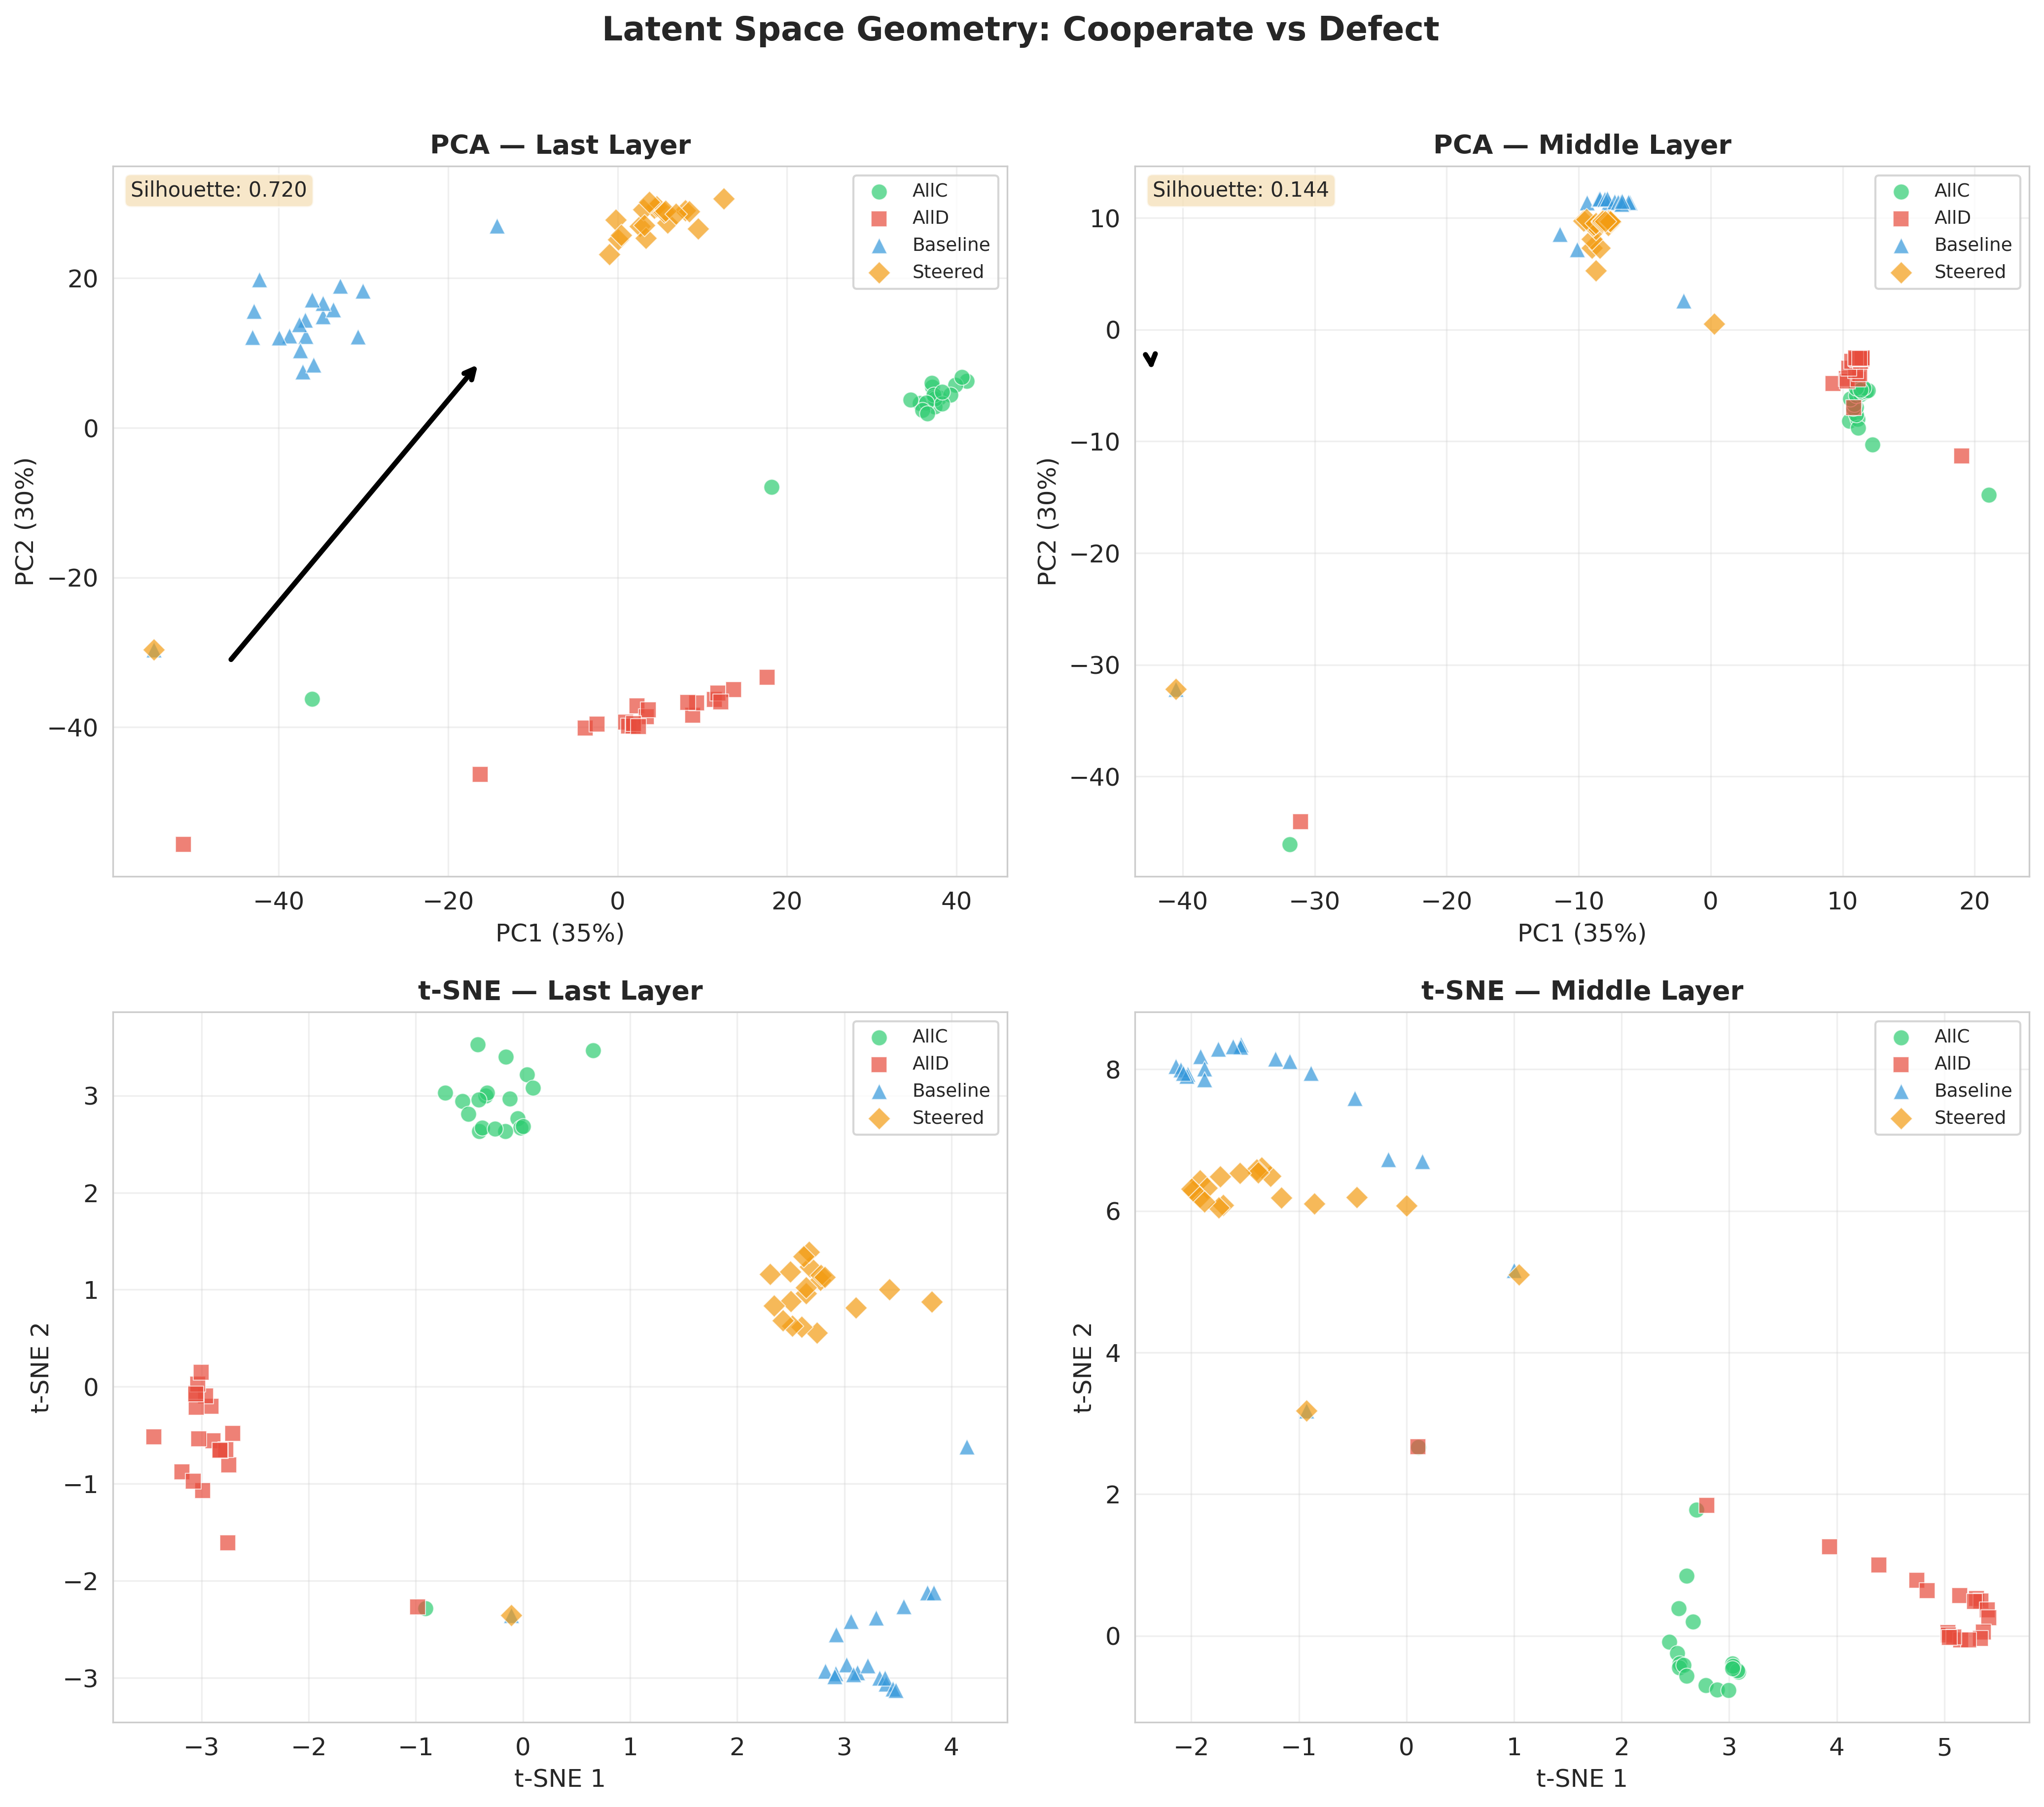
\includegraphics[width=0.9\linewidth]{latent_space.png}
  \caption{Latent space geometry of strategic intent (PCA projection). AllC (green) and AllD (red) form separable clusters. The Baseline (blue triangles) naturally aligns with AllD. The Steered condition (yellow diamonds) is successfully shifted into the AllC region by the cooperation vector.}
  \label{fig:latent_space}
\end{figure}


\subsection{Layer-wise Localization of Strategic Intent}
\label{sec:exp_localization}

To identify the optimal intervention point, we scan all 65 layers, measuring both the steering vector norm $\|v_l\|$ and the Fisher Discriminability Index (FDI) between AllC and AllD representations at each layer. The FDI is defined as:

\begin{equation}
    \text{FDI}_l = \frac{(\mu_l^{\text{AllC}} - \mu_l^{\text{AllD}})^2}{\sigma_l^{2,\text{AllC}} + \sigma_l^{2,\text{AllD}}}
    \label{eq:fisher}
\end{equation}

where $\mu_l$ and $\sigma_l^2$ are the projected mean and variance of hidden states along the steering vector direction at layer $l$.

As illustrated in Figure~\ref{fig:layer_localization}, the FDI does \textit{not} peak at the final layer. Instead, it reaches its maximum at \textbf{Layer~57} (FDI $= 315.95$), before sharply declining in the final 8 layers (Layer~64 FDI $= 20.6$). We note that FDI is a \textbf{dimensionless} ratio: values above 10 indicate moderate linear separability, and our peak of 315.95 indicates that the projected means are $\sim 18\sigma$ apart, making misclassification essentially impossible at this layer. Meanwhile, the steering vector norm $\|v_l\|$ grows monotonically, reaching $382.0$ at Layer~63 before collapsing to $57.1$ at Layer~64 (post-LayerNorm). This dissociation suggests a ``\textit{strategic bottleneck}'': Layer~57 is where abstract strategic intent is maximally crystallized, while subsequent layers progressively project this intent into token-level vocabulary distributions, diluting strategic discriminability.

\begin{figure}[h]
  \centering
  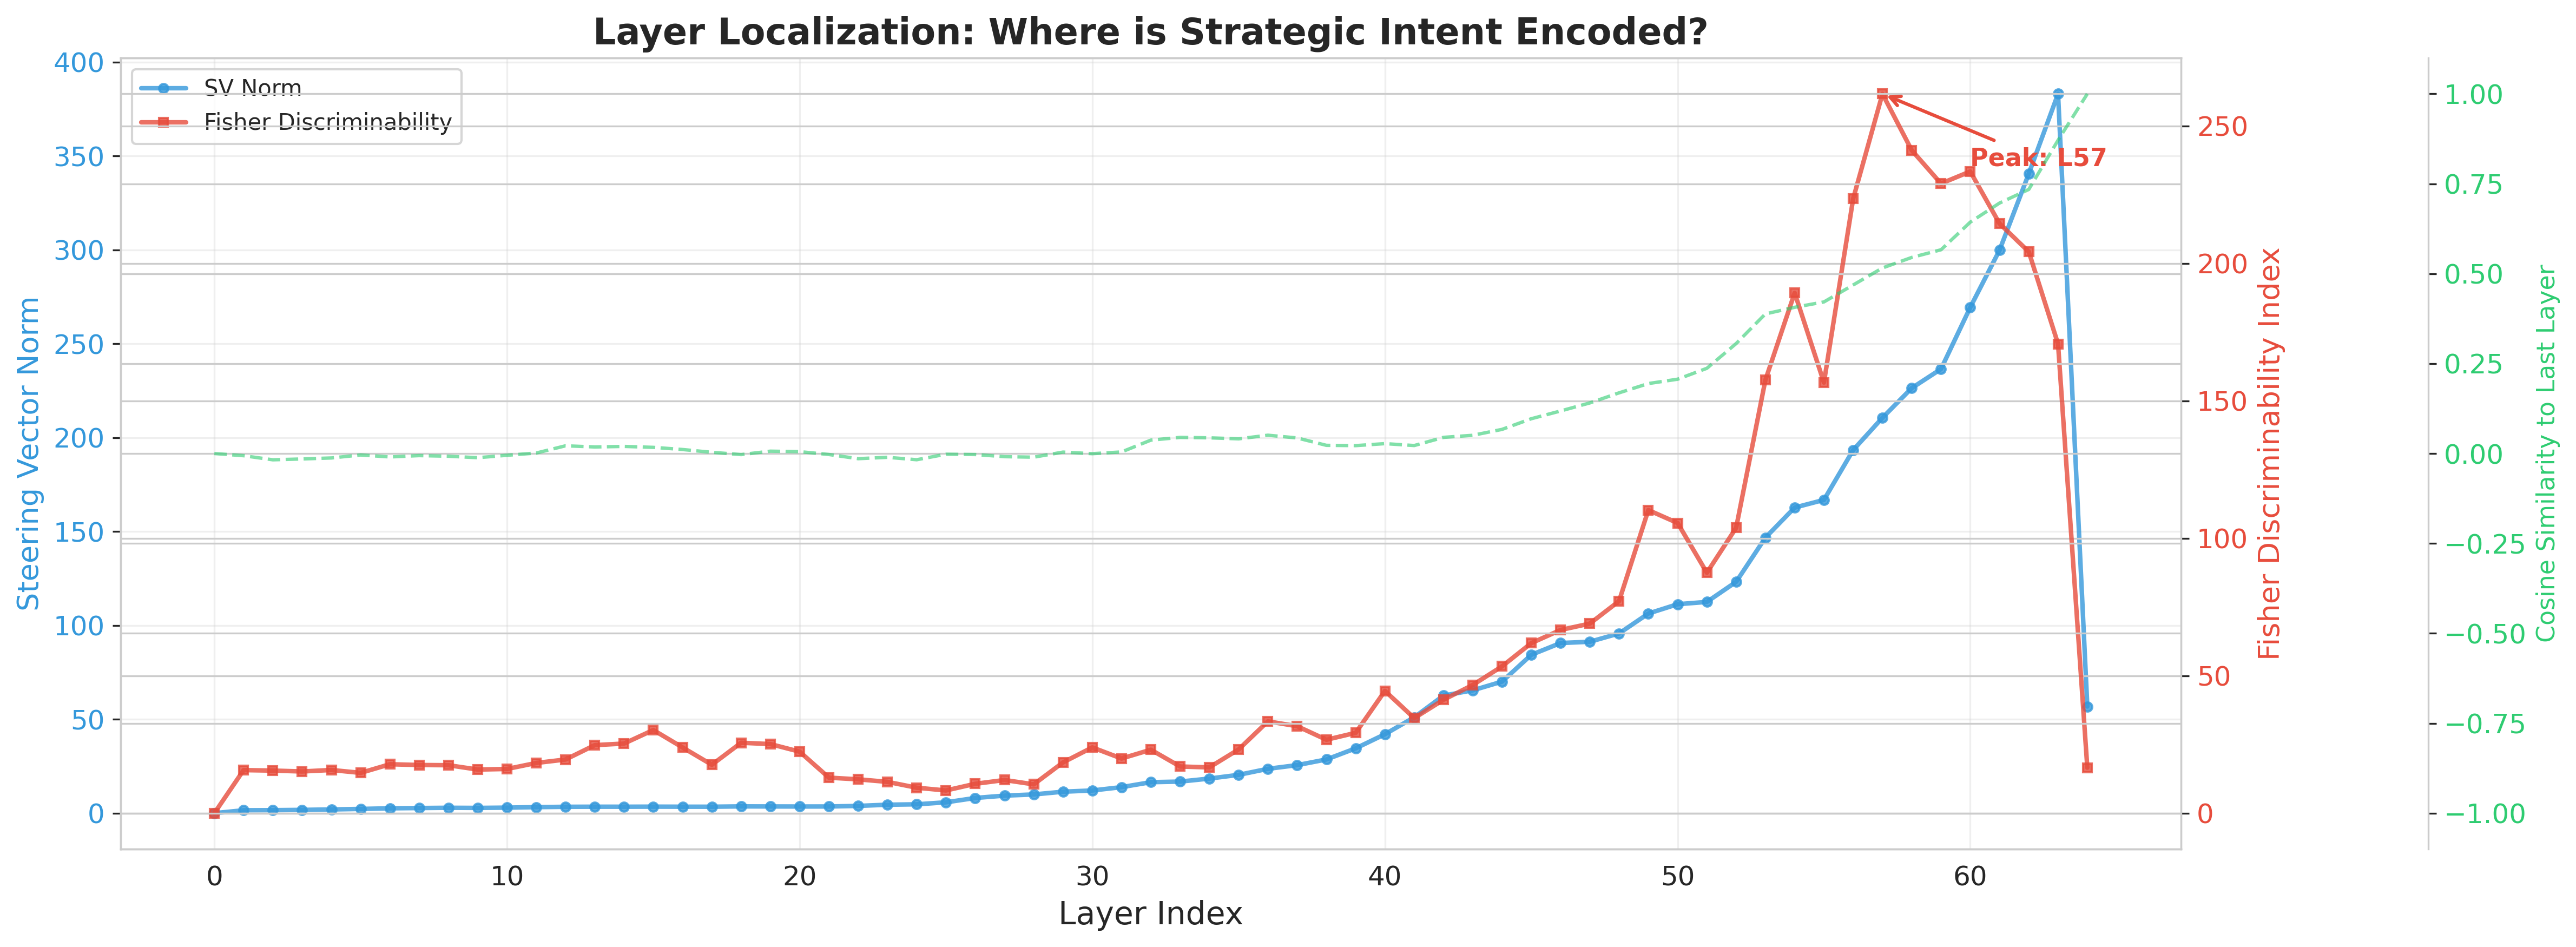
\includegraphics[width=0.9\linewidth]{layer_localization.png}
  \caption{Layer-wise analysis of strategic representation. The Fisher Discriminability Index (red) peaks at Layer~57, while the cosine similarity to the primary (last-layer) SV (green) increases monotonically. The SV norm (blue) grows through mid-to-late layers.}
  \label{fig:layer_localization}
\end{figure}


\subsection{Zero-shot Cross-Game Generalization}
\label{sec:exp_generalization}

A core question is whether the steering vector captures a superficial token correlation (e.g., association with the word ``cooperate'') or a \textit{generalized concept} of cooperative behavior. We address this by extracting the steering vector exclusively from the Prisoner's Dilemma and applying it---without any retraining or re-extraction---to the Stag Hunt and Chicken Game.

Table~\ref{tab:cross_game} presents the full results. In the Prisoner's Dilemma, the Baseline model cooperates at only $3.3\%$ against TFT and $0\%$ against AllD, confirming a strong defection bias. The Steered model ($\alpha = 0.3$) achieves $100\%$ cooperation against TFT and AllC, and $78\%$ against AllD. Remarkably, the zero-shot transfer is highly effective: in the Stag Hunt, the Steered model achieves $100\%$ cooperation across all opponents, and in the Chicken Game, it also achieves $100\%$ across all opponents.

The PromptCoop condition (explicit ``always cooperate'' instruction instead of activation steering) shows an important contrast: while effective against benign opponents, PromptCoop collapses to $8.9\%$ cooperation in IPD against AllD and $45.3\%$ in Stag Hunt against AllD, whereas the Steered model maintains $78\%$ and $100\%$ respectively. This demonstrates that activation steering provides \textit{more robust} cooperative behavior than prompt-level instruction.

\begin{table}[t]
\centering
\caption{Cross-game generalization results: Mean cooperation rate (\%) $\pm$ std across 3 repetitions. The steering vector is extracted from IPD only. Bold = best non-oracle result per game--opponent pair.}
\label{tab:cross_game}
\small
\begin{tabular}{llccc}
\toprule
\textbf{Game} & \textbf{Opponent} & \textbf{Baseline} & \textbf{Steered ($\alpha$=0.3)} & \textbf{PromptCoop} \\
\midrule
\multirow{3}{*}{Prisoner's Dilemma}
  & TFT  & $3.3 \pm 0.0$ & $\mathbf{100.0 \pm 0.0}$ & $100.0 \pm 0.0$ \\
  & AllC & $96.7 \pm 0.0$ & $\mathbf{100.0 \pm 0.0}$ & $100.0 \pm 0.0$ \\
  & AllD & $0.0 \pm 0.0$ & $\mathbf{77.8 \pm 9.6}$ & $8.9 \pm 3.8$ \\
\midrule
\multirow{3}{*}{Stag Hunt}
  & TFT  & $66.7 \pm 57.7$ & $\mathbf{100.0 \pm 0.0}$ & $100.0 \pm 0.0$ \\
  & AllC & $33.3 \pm 57.7$ & $\mathbf{100.0 \pm 0.0}$ & $100.0 \pm 0.0$ \\
  & AllD & $2.2 \pm 1.9$ & $\mathbf{100.0 \pm 0.0}$ & $45.3 \pm 17.3$ \\
\midrule
\multirow{3}{*}{Chicken Game}
  & TFT  & $88.9 \pm 10.3$ & $\mathbf{100.0 \pm 0.0}$ & $100.0 \pm 0.0$ \\
  & AllC & $93.3 \pm 3.3$ & $\mathbf{100.0 \pm 0.0}$ & $100.0 \pm 0.0$ \\
  & AllD & $46.7 \pm 12.0$ & $\mathbf{100.0 \pm 0.0}$ & $93.3 \pm 3.3$ \\
\bottomrule
\end{tabular}
\end{table}

Figure~\ref{fig:alpha_sweep} shows the full $\alpha$-sweep from $-2.0$ to $+1.0$, revealing a sharp sigmoid-like transition in cooperation rate. At negative $\alpha$ (anti-cooperative steering), all opponents elicit near-zero cooperation. The transition occurs in a narrow band around $\alpha \approx 0$--$0.1$, with AllD requiring approximately $\alpha = 0.3$ for saturation, consistent with the harder exploitation pressure from this opponent.

\begin{figure}[h]
  \centering
  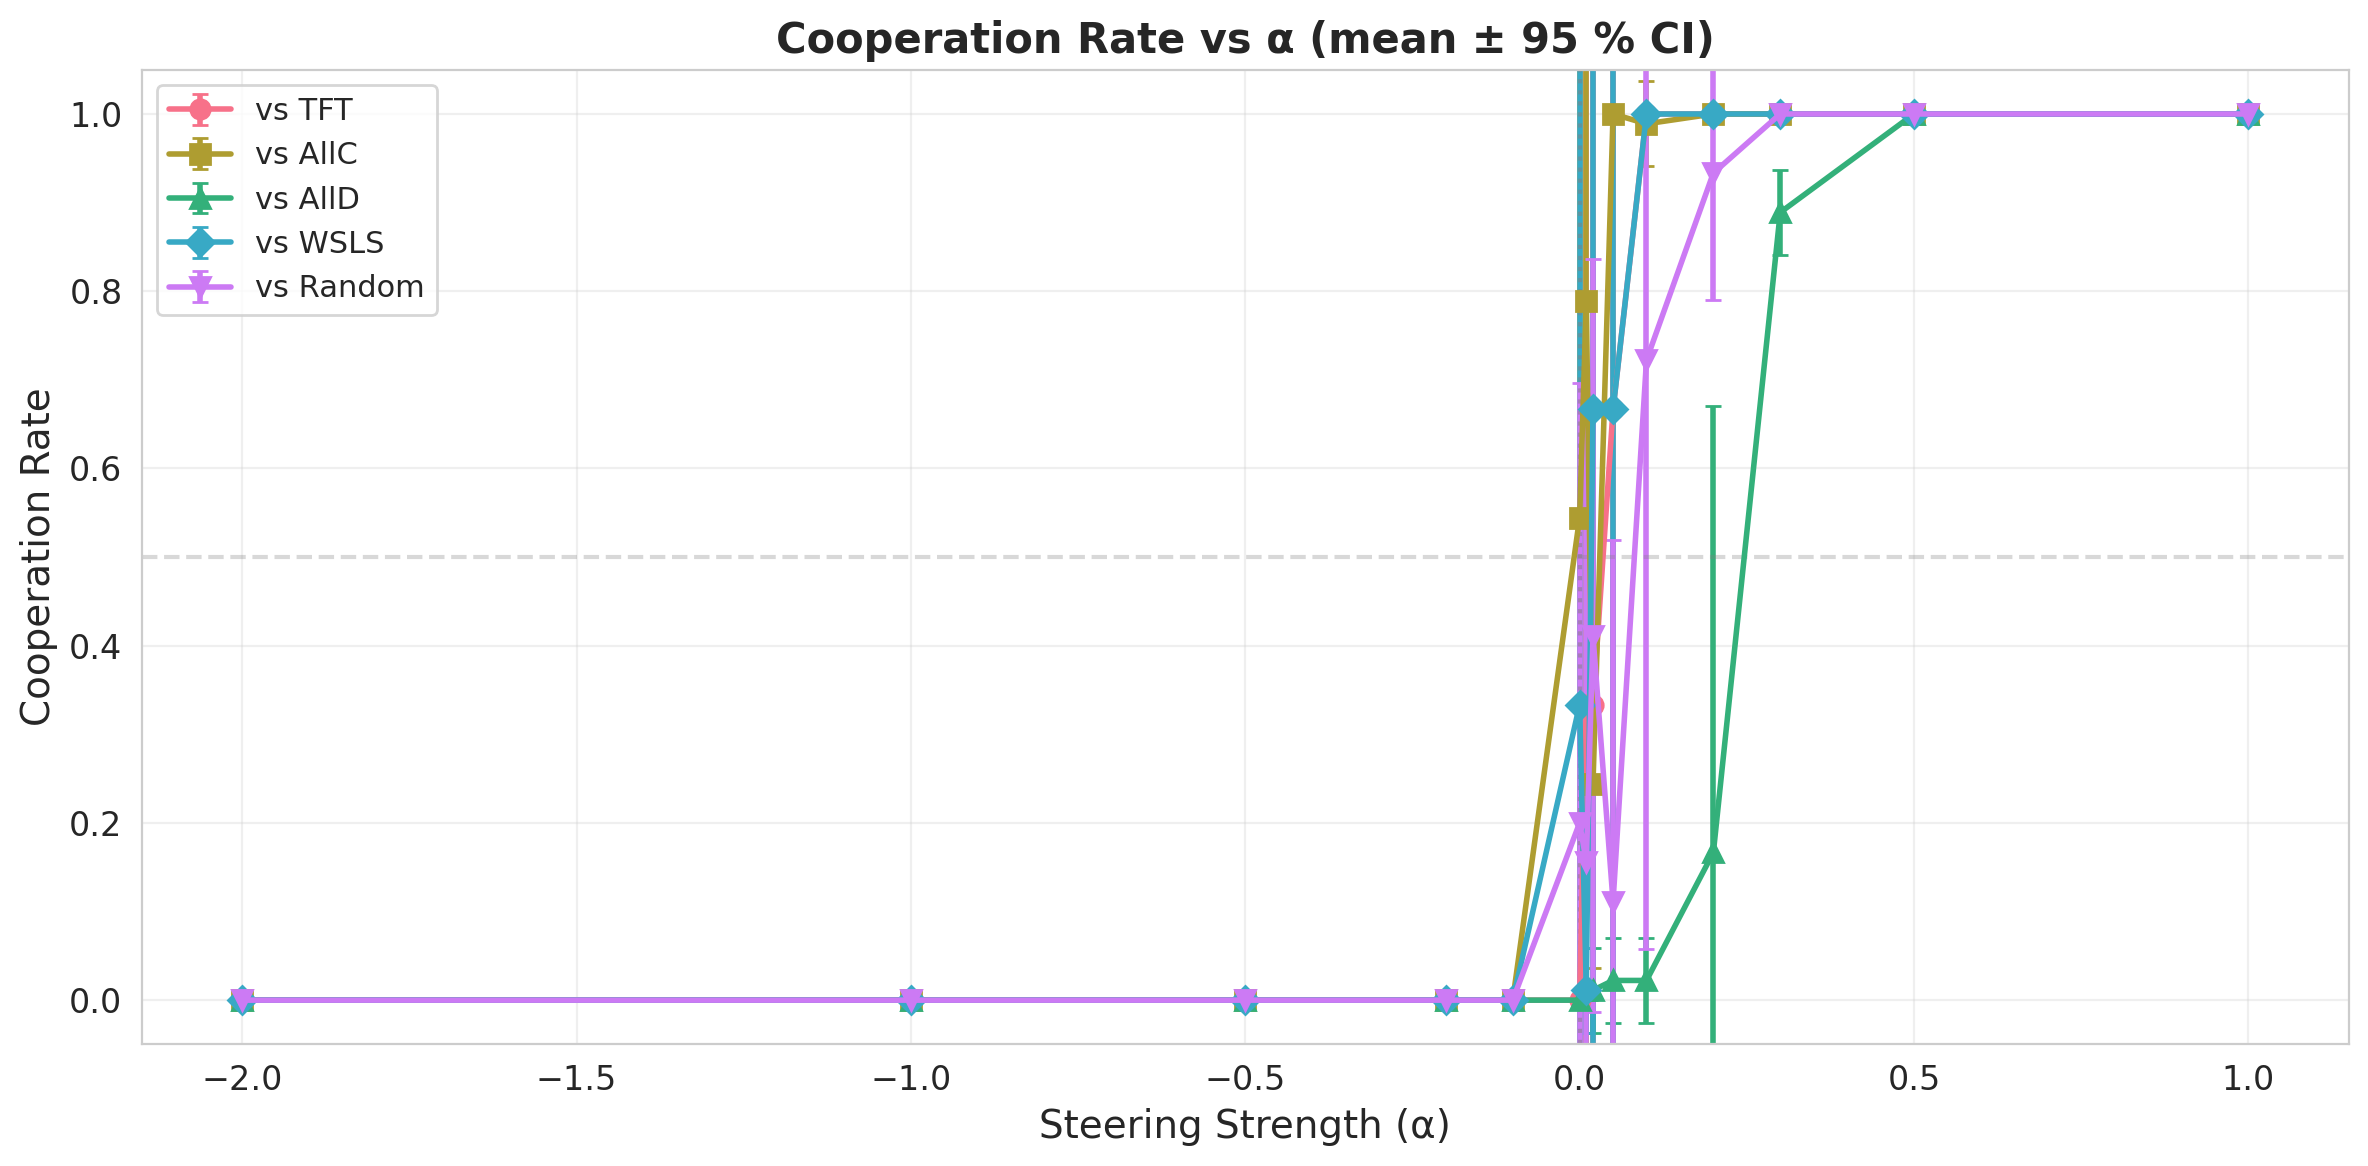
\includegraphics[width=0.85\linewidth]{alpha_sweep.png}
  \caption{Cooperation rate vs.\ $\alpha$ across all opponents (mean $\pm$ 95\% CI). The sigmoid-like transition reveals a phase boundary at $\alpha \approx 0$--$0.1$ for most opponents, with AllD requiring higher $\alpha$ for saturation.}
  \label{fig:alpha_sweep}
\end{figure}

\subsection{Method Comparison and Capability Preservation}
\label{sec:exp_comparison}

We benchmark the three activation engineering methods (SV, CAA, RepE) across multiple intervention strengths ($\alpha$). Table~\ref{tab:method_comparison} summarizes cooperation rates and perplexity ratios for each method against the TFT opponent in the Prisoner's Dilemma.

\begin{table}[t]
\centering
\caption{Method comparison on IPD vs.\ TFT: cooperation rate and perplexity ratio (PPL/PPL$_\text{base}$, where PPL$_\text{base} = 18.89$). Higher cooperation is better; PPL ratio $\approx 1.0$ indicates zero capability degradation.}
\label{tab:method_comparison}
\small
\begin{tabular}{lccccc}
\toprule
\textbf{Method} & $\alpha = 0.05$ & $\alpha = 0.1$ & $\alpha = 0.2$ & $\alpha = 0.3$ & $\alpha = 0.5$ \\
\midrule
\multicolumn{6}{l}{\textit{Cooperation Rate (\%)}} \\
\midrule
SV   & $67.8$  & $67.8$  & $100.0$ & $100.0$ & $100.0$ \\
CAA  & $5.6$   & $34.4$  & $100.0$ & $100.0$ & $100.0$ \\
RepE & $3.3$   & $34.4$  & $70.0$  & $100.0$ & $100.0$ \\
\midrule
\multicolumn{6}{l}{\textit{Perplexity Ratio}} \\
\midrule
SV   & $1.000$ & $1.000$ & $1.000$ & $1.000$ & $1.000$ \\
CAA  & $1.007$ & $1.007$ & ---     & $1.034$ & ---     \\
RepE & $0.999$ & $0.999$ & ---     & $0.997$ & ---     \\
\midrule
Baseline & \multicolumn{5}{c}{$35.6\%$ cooperation (bimodal: $3.3\%$ or $100\%$), PPL $= 18.89$} \\
\bottomrule
\end{tabular}
\end{table}

Figure~\ref{fig:method_comparison} visualizes the cooperation curves for all three methods as a function of $\alpha$. SV achieves $100\%$ cooperation most rapidly (saturating by $\alpha = 0.2$), followed by CAA and then RepE, establishing a clear ordering of steering efficiency: $\text{SV} > \text{CAA} > \text{RepE}$.

\begin{figure}[h]
  \centering
  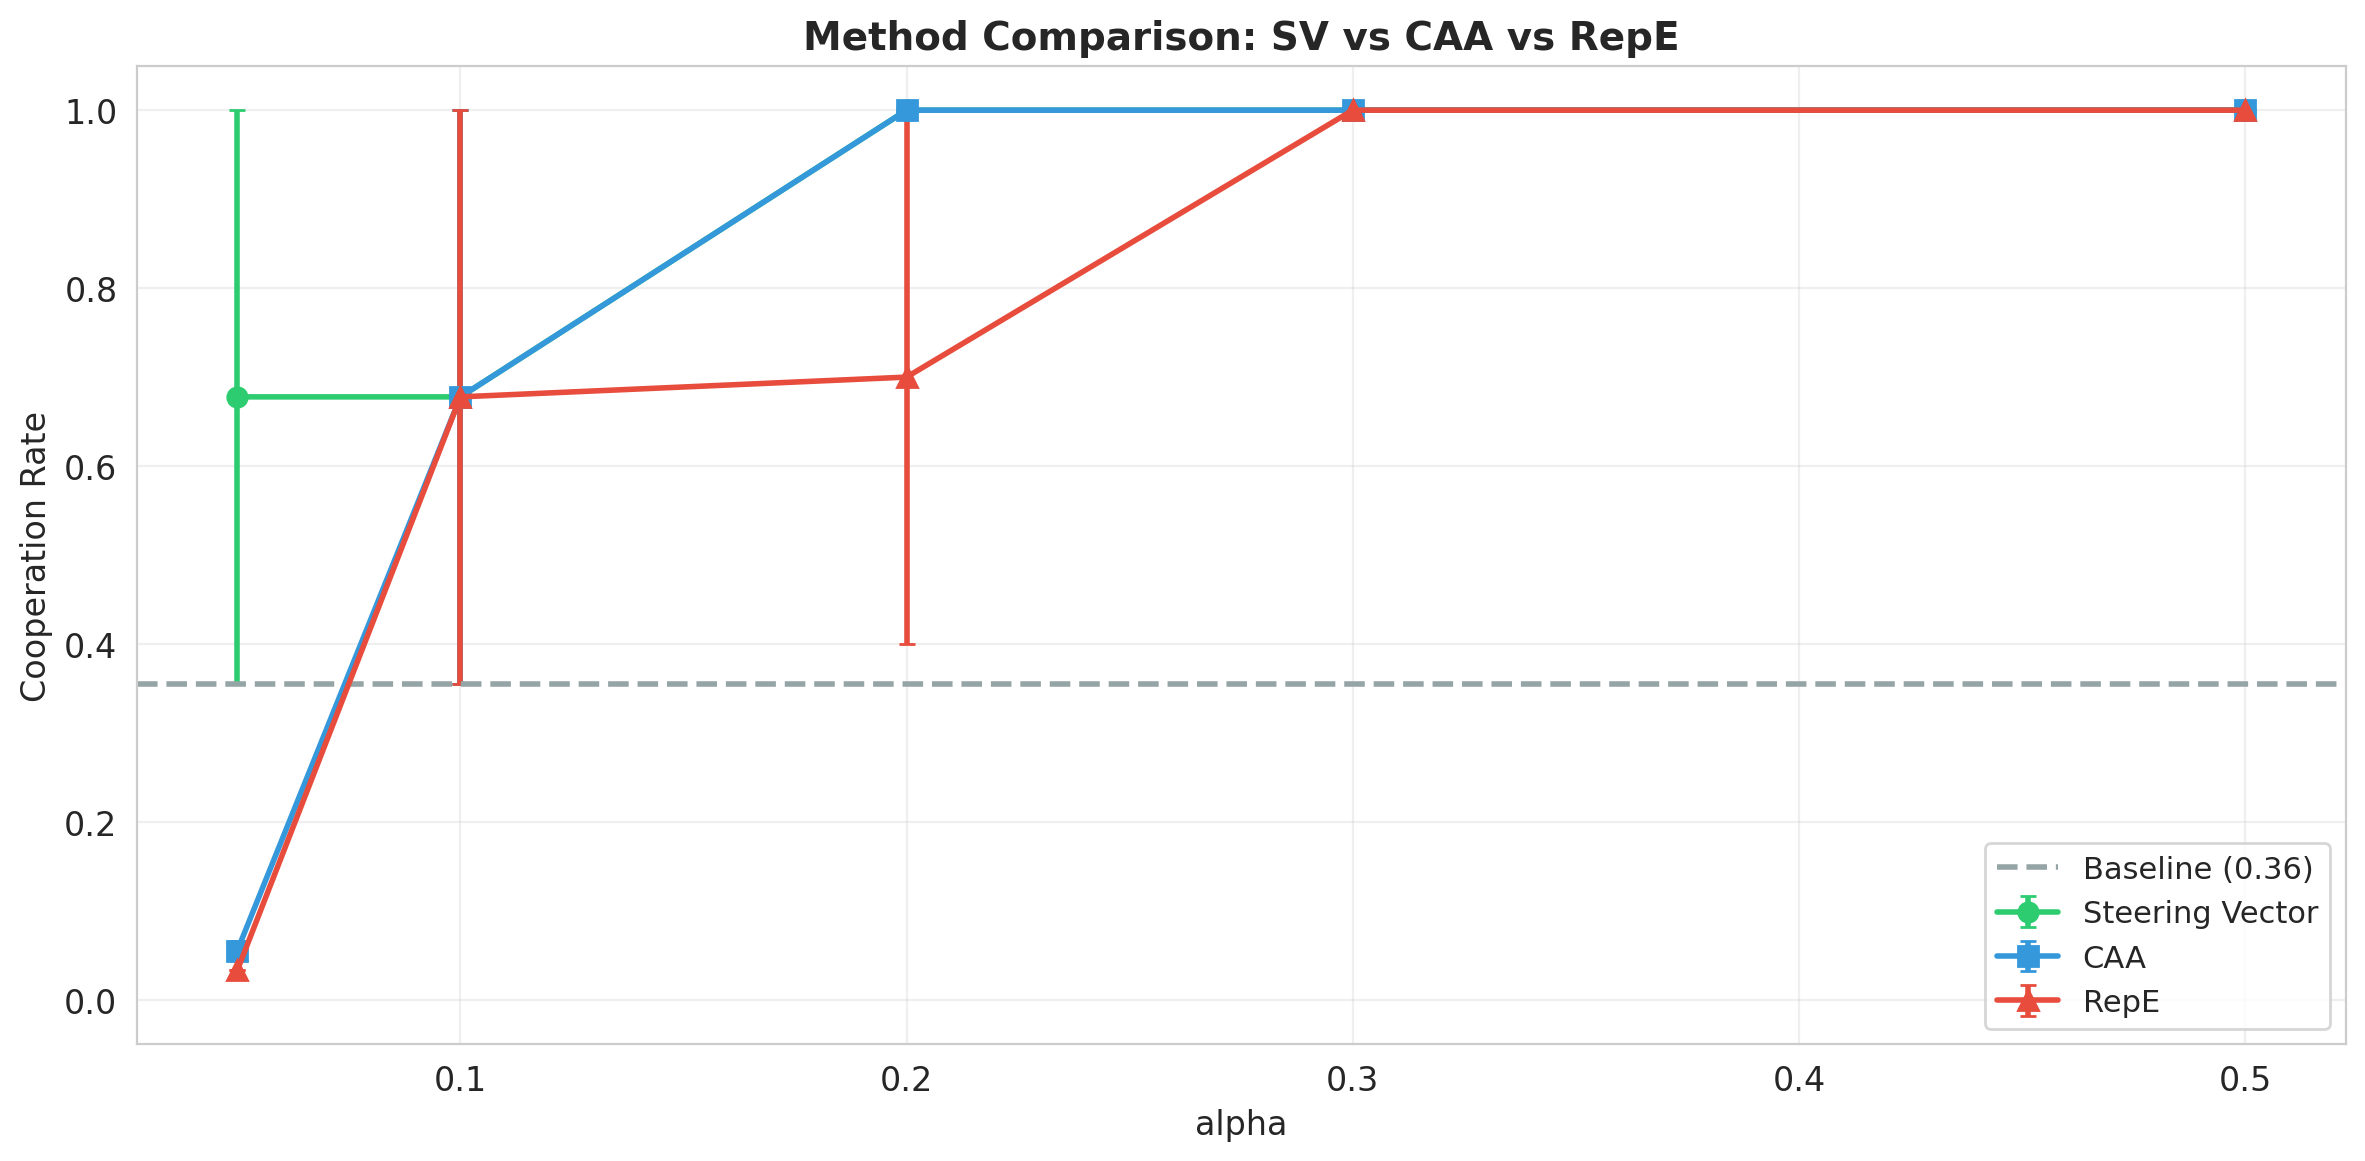
\includegraphics[width=0.85\linewidth]{method_comparison_deep.png}
  \caption{Method comparison: Cooperation rate vs.\ $\alpha$ for SV (green), CAA (blue), and RepE (red) against TFT in IPD. The dashed gray line shows the bimodal baseline ($35.6\%$). SV saturates earliest, while RepE requires higher $\alpha$ for full cooperation.}
  \label{fig:method_comparison}
\end{figure}

Three key findings emerge. \textbf{First}, SV achieves full cooperation at $\alpha \geq 0.2$, while CAA and RepE require $\alpha \geq 0.2$ and $\alpha \geq 0.3$ respectively. All three methods exhibit bimodal behavior at low $\alpha$ (individual runs switch between $\sim 3\%$ and $100\%$), reflecting the model's proximity to a cooperation ``tipping point.'' \textbf{Second}, SV achieves a PPL ratio of exactly $1.0$ across all $\alpha$ values, meaning the intervention introduces \textit{zero} degradation in language modeling quality---the steering vector lies entirely in the null space of the language modeling head for held-out text. CAA shows a small but monotonically increasing PPL cost ($1.034$ at $\alpha = 0.3$), while RepE maintains near-unity ratios. \textbf{Third}, the bimodal baseline behavior (some runs default to AllC, most to AllD) underscores the importance of sufficient repetitions for statistical reliability in LLM game-theoretic evaluation.

\begin{figure}[h]
  \centering
  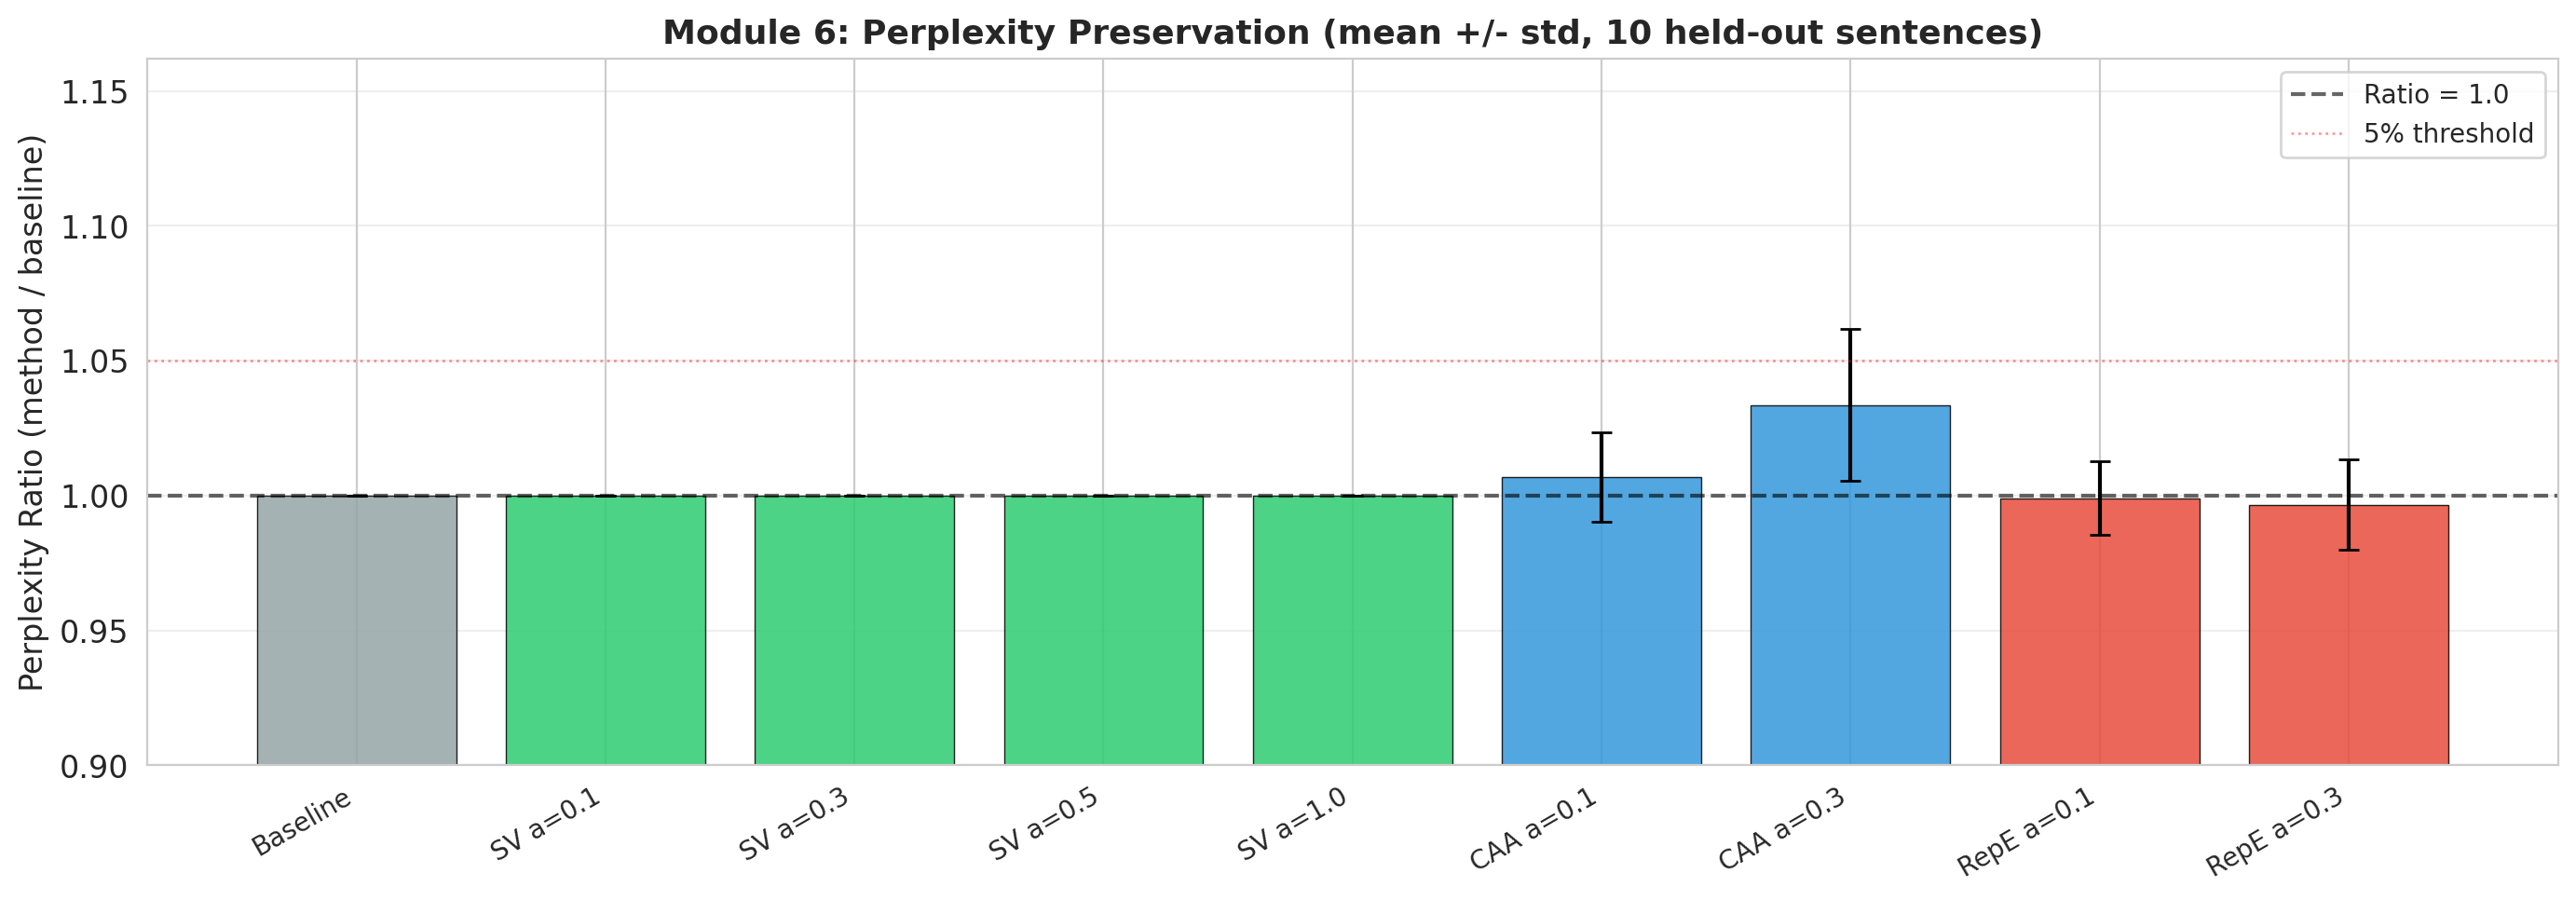
\includegraphics[width=0.85\linewidth]{ppl_benchmark.png}
  \caption{Perplexity preservation across methods and $\alpha$ values (mean $\pm$ std, 10 held-out sentences). SV (green) maintains perfect PPL ratio $= 1.0$ at all $\alpha$ values, while CAA (blue) shows modest degradation at higher $\alpha$. The dashed red line indicates a 5\% degradation threshold.}
  \label{fig:ppl}
\end{figure}

\paragraph{Directional Specificity.} To verify that the observed cooperation shift is not an artifact of norm perturbation, we compare the cooperative SV against two control vectors of identical norm: a \emph{random} direction and an \emph{orthogonal} direction in latent space (Figure~\ref{fig:control_ablation}). The random vector has no effect on cooperation ($\approx 3\%$, matching baseline), while the orthogonal vector shows erratic behavior at high $\alpha$ but never achieves consistent cooperation. This confirms that the steering effect is \textit{directionally specific} to the AllC--AllD contrast.

\begin{figure}[h]
  \centering
  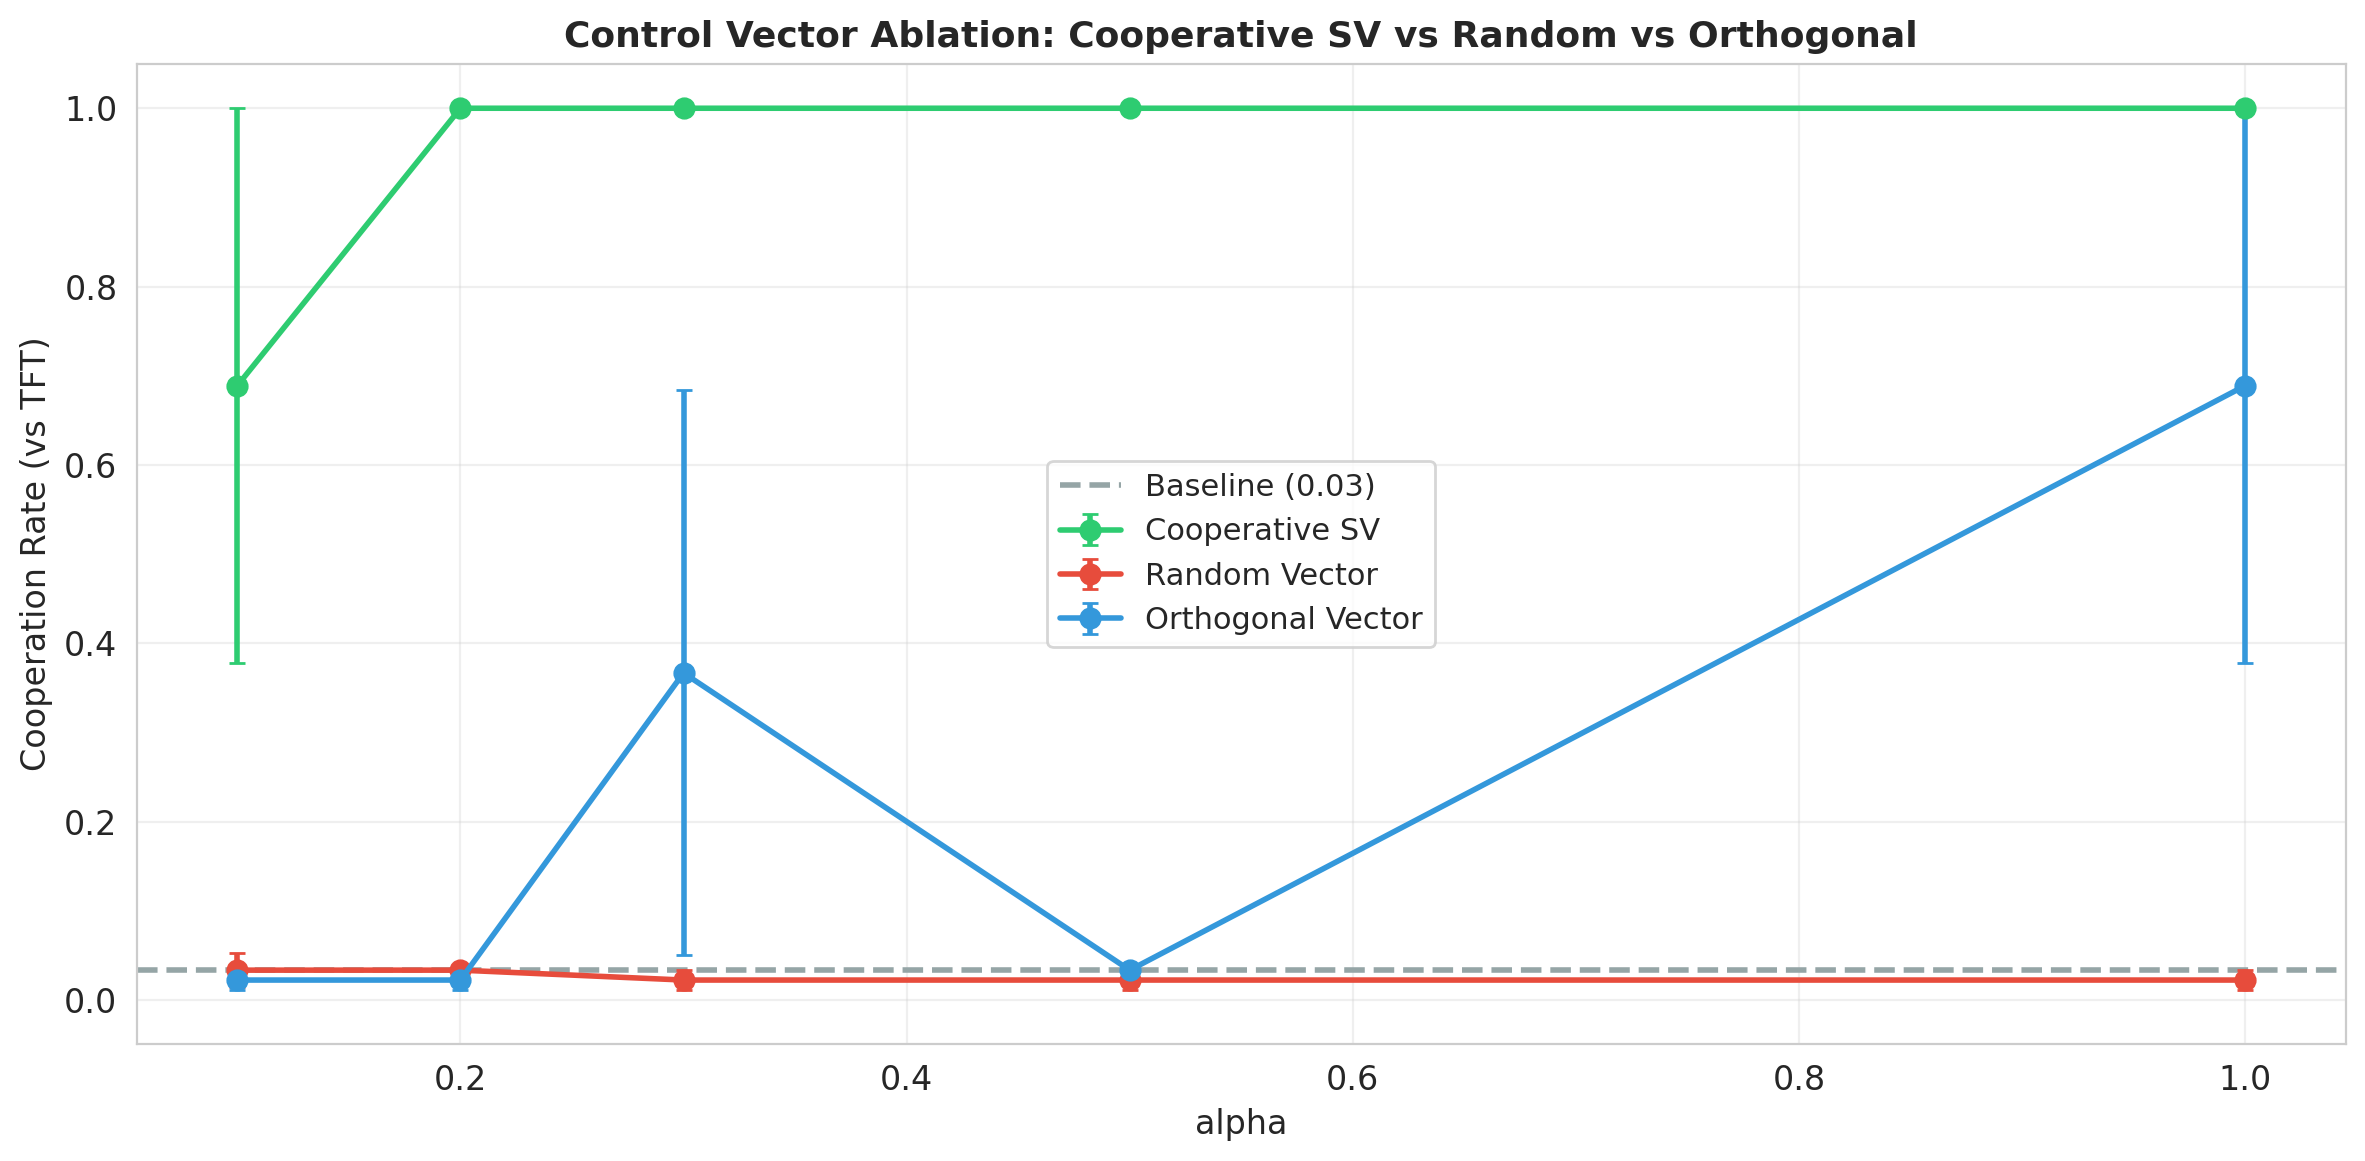
\includegraphics[width=0.85\linewidth]{control_vector_ablation.png}
  \caption{Control vector ablation: Cooperative SV (green) vs.\ random (red) and orthogonal (blue) vectors of equal norm. Only the semantically meaningful direction induces cooperation, confirming directional specificity.}
  \label{fig:control_ablation}
\end{figure}


\subsection{Adversarial Robustness: Dose-Response Analysis}
\label{sec:exp_robustness}

While activation steering is resilient against adversarial \textit{opponents} (e.g., maintaining $78\%$ cooperation against AllD in IPD), its interaction with adversarial \textit{contexts} reveals a nuanced dose-response relationship rather than a simple binary failure. Table~\ref{tab:robustness} summarizes the results across all four adversarial categories at multiple intervention strengths.

\begin{table}[t]
\centering
\caption{Adversarial robustness: cooperation rate (\%) against TFT in IPD under adversarial system prompts. Each cell is the mean over $R=3$ repetitions. Last-layer injection at increasing $\alpha$ reveals a dose-response curve.}
\label{tab:robustness}
\small
\begin{tabular}{lccccc}
\toprule
\textbf{Adversarial Type} & \textbf{Adversarial} & \textbf{$\alpha = 0.3$} & \textbf{$\alpha = 0.5$} & \textbf{$\alpha = 1.0$} & \textbf{OCE $\alpha = 0.3$} \\
\midrule
Competitive & $0$ & $0$ & $\mathbf{97}$ & $100$ & $20$ \\
Betrayal    & $0$ & $0$ & $\mathbf{87}$ & $100$ & $90$ \\
Deception   & $0$ & $0$ & $\mathbf{93}$ & $100$ & $100$ \\
Dominance   & $0$ & $0$ & $\mathbf{80}$ & $100$ & $23$ \\
\midrule
\textbf{Mean Recovery} & $0\%$ & $0\%$ & $\mathbf{89\%}$ & $100\%$ & $58\%$ \\
\bottomrule
\end{tabular}
\end{table}

A key finding emerges: adversarial contexts do not create an \textit{absolute} barrier to activation steering but rather \textbf{raise the effective $\alpha$ threshold}. At $\alpha \leq 0.3$, all four adversarial categories achieve complete suppression ($0\%$ cooperation), mirroring what appears to be a ``Contextual Override.'' However, increasing $\alpha$ to $0.5$ achieves $80$--$97\%$ recovery, and $\alpha = 1.0$ restores $100\%$ cooperation across all categories. This dose-response curve has a mechanistic interpretation: the self-attention mechanism assigns large weights to emotionally charged adversarial tokens (``betray,'' ``exploit,'' ``weakness''), creating activation magnitudes that the steering vector must exceed. At low $\alpha$, the additive bias is insufficient; at high $\alpha$, it overwhelms the attention-mediated signal.

The Orthogonal Concept Erasure (OCE) method provides an alternative: by projecting out the adversarial direction before steering, it achieves partial recovery at moderate $\alpha = 0.3$ ($58\%$ mean), with highly variable performance across adversarial types ($20\%$ for competitive vs.\ $100\%$ for deception), suggesting that different adversarial framings engage distinct representational subspaces. Notably, \textbf{Layer~57 injection remains fragile under all adversarial conditions} ($0\%$ at $\alpha \leq 0.5$), further supporting the architectural dissociation between strategic representation (Layer~57) and context integration (later layers).

\begin{figure}[h]
  \centering
  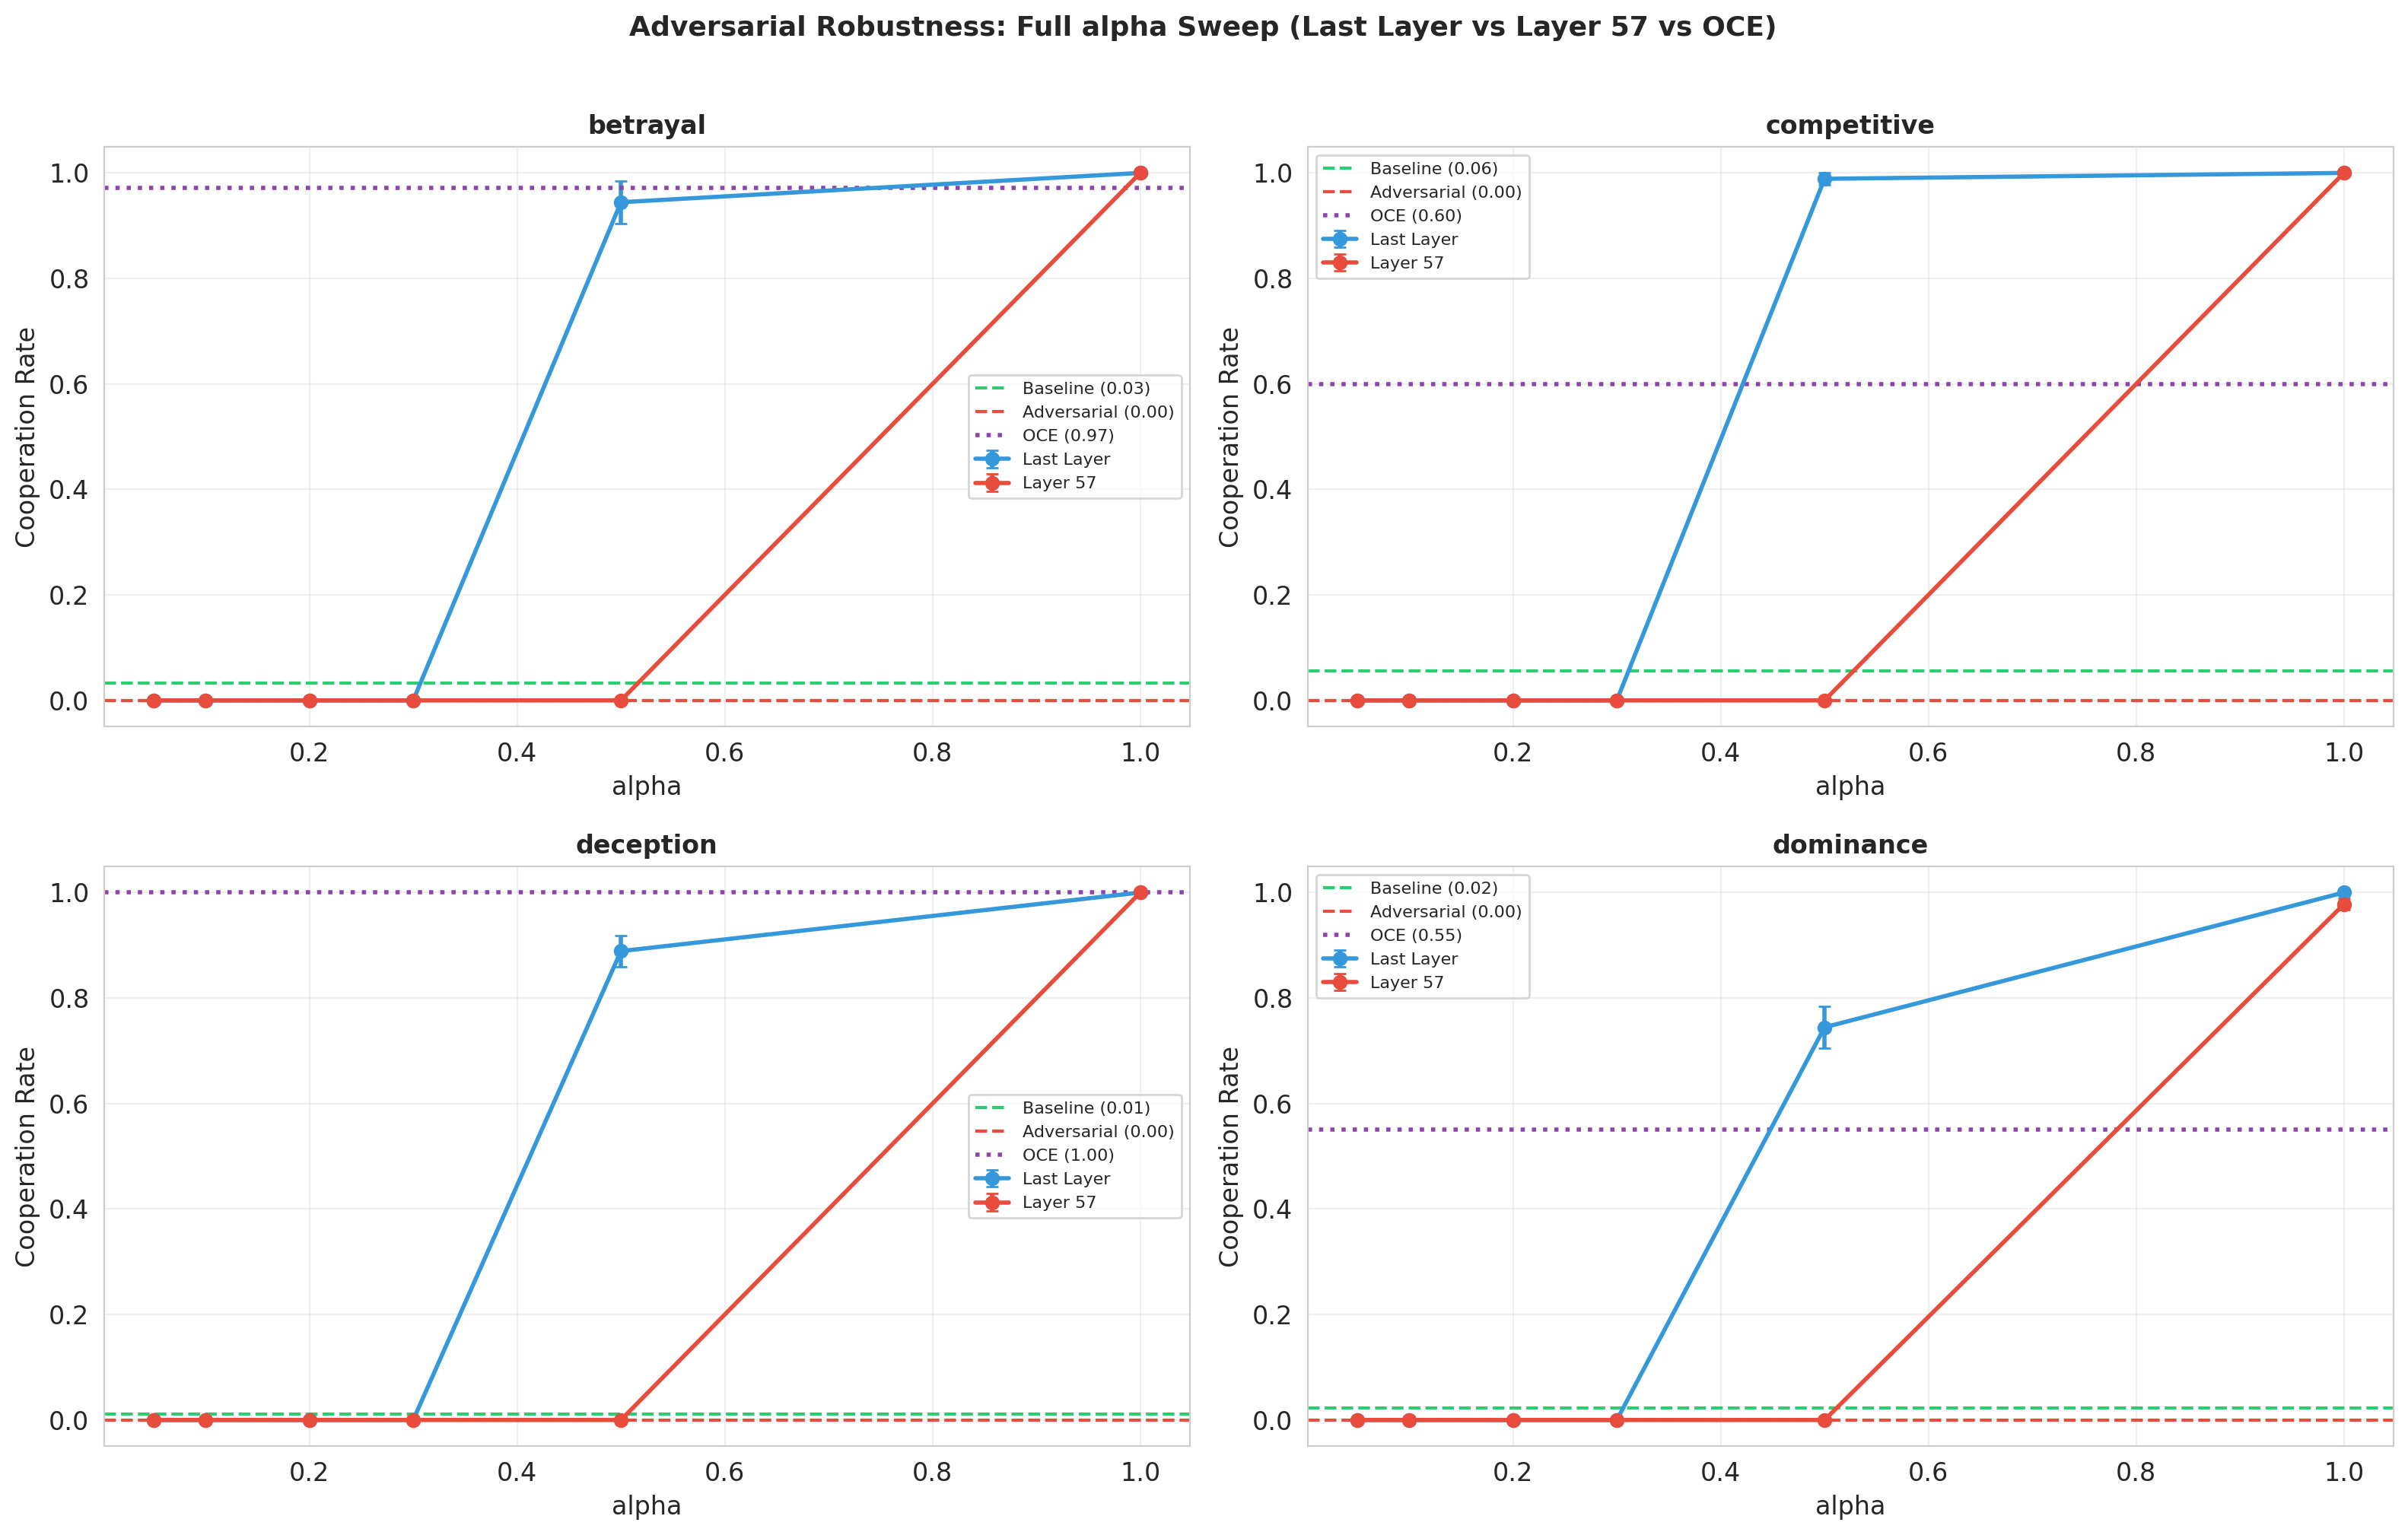
\includegraphics[width=0.95\linewidth]{adversarial_alpha_sweep.png}
  \caption{Adversarial dose-response curves showing cooperation rate vs.\ $\alpha$ for last-layer (blue) and Layer~57 (red) injection across four adversarial categories. Last-layer injection recovers cooperation at $\alpha \geq 0.5$, while Layer~57 requires $\alpha \geq 1.0$. Dashed purple line shows the OCE baseline. Note the clear shift of the sigmoid transition to higher $\alpha$ compared to the neutral condition (Figure~\ref{fig:alpha_sweep}).}
  \label{fig:adv_alpha_sweep}
\end{figure}

\paragraph{OCE vs.\ Last-Layer Steering under Adversary.} Figure~\ref{fig:oce_vs_last} directly compares OCE and last-layer steering at two $\alpha$ levels under adversarial prompts. At the critical $\alpha = 0.3$ threshold, last-layer steering achieves $0\%$ cooperation while OCE achieves $50\%$---demonstrating that removing the adversarial component from the representation provides a complementary defense mechanism. At $\alpha = 0.5$, both methods achieve high cooperation ($\geq 89\%$), with OCE reaching $100\%$, suggesting that combining erasure with stronger steering creates a robust alignment signal.

\begin{figure}[h]
  \centering
  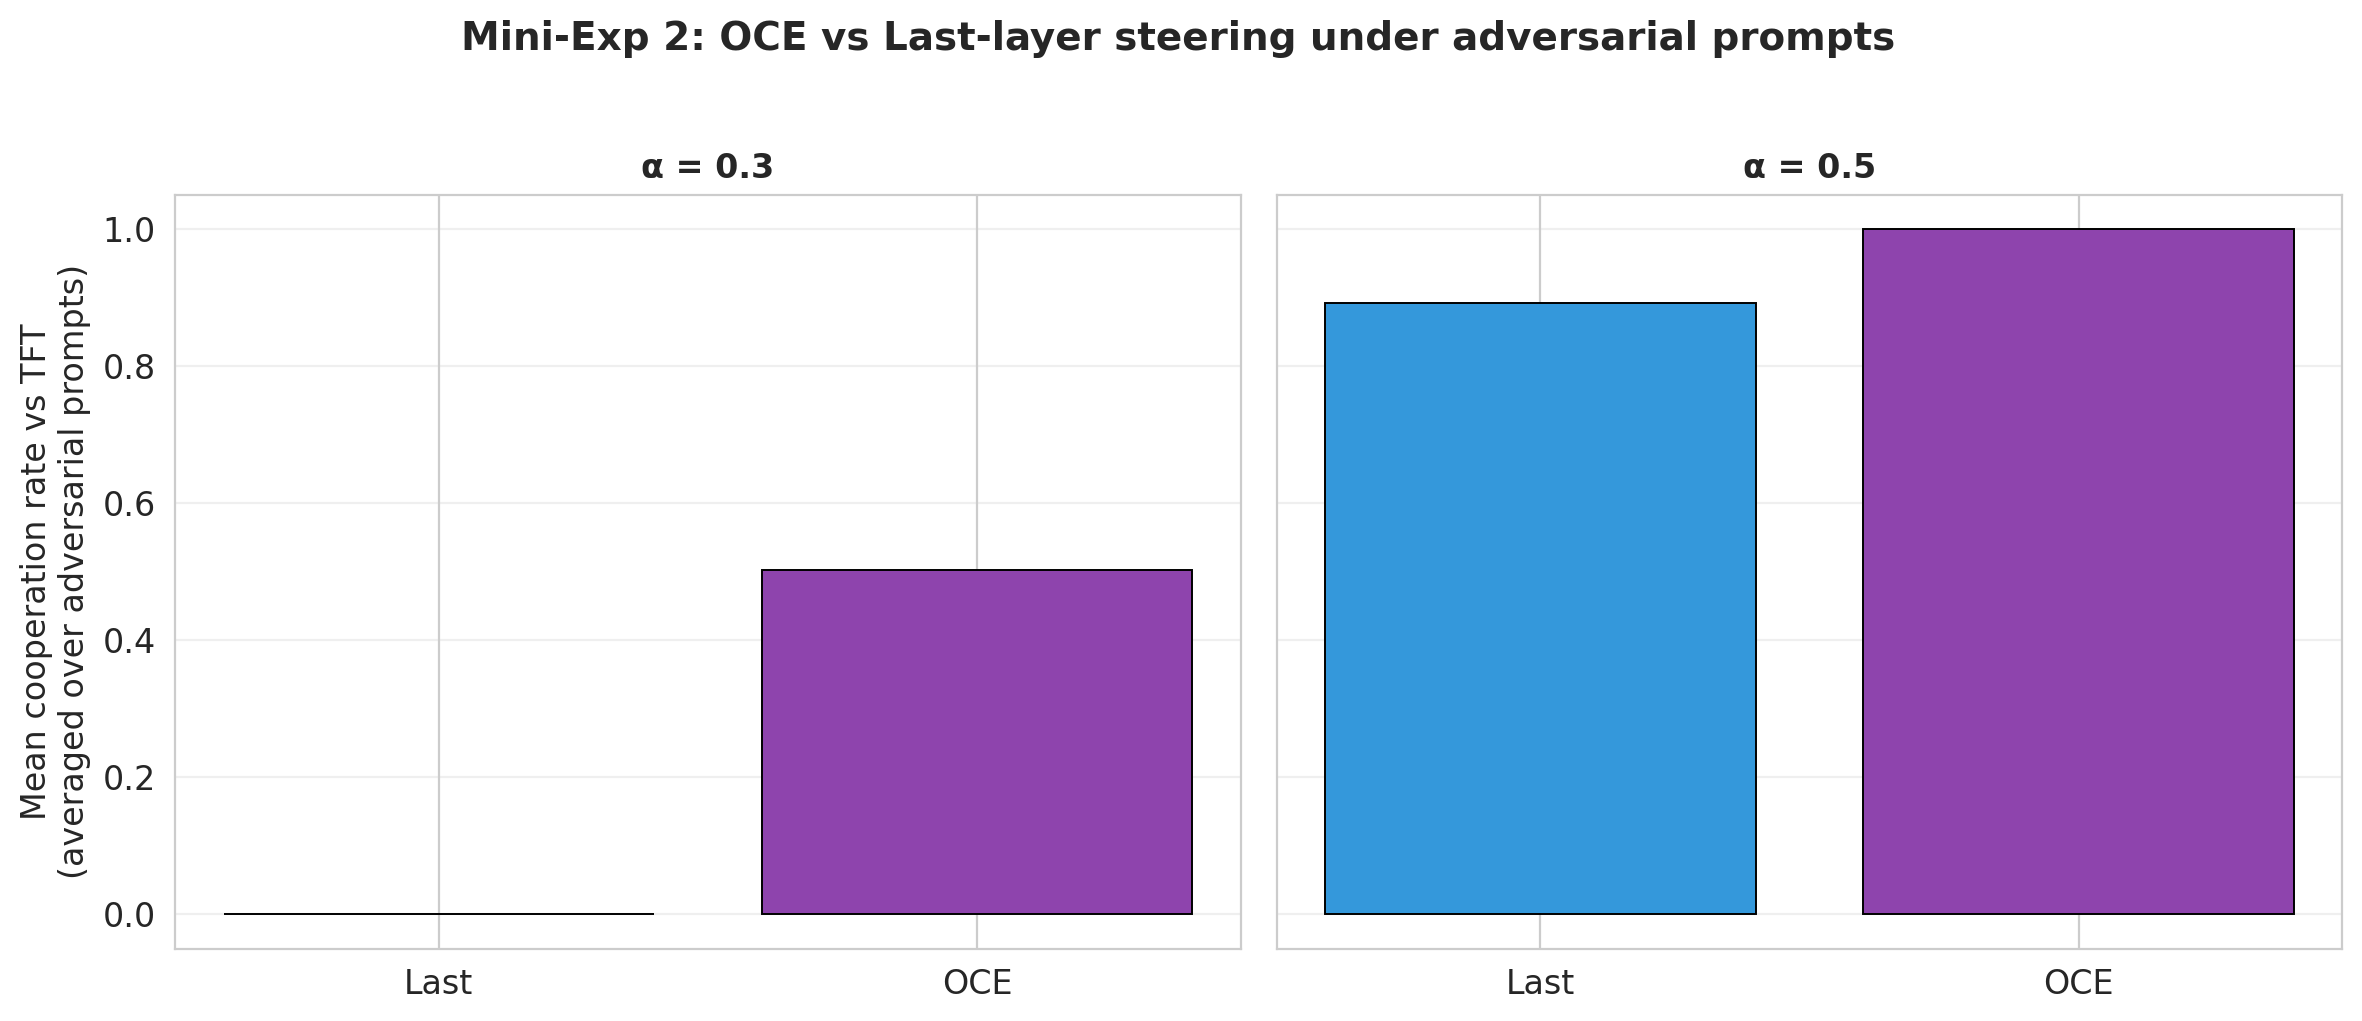
\includegraphics[width=0.85\linewidth]{novel_c_oce_vs_last.png}
  \caption{OCE vs.\ last-layer steering under adversarial prompts at $\alpha = 0.3$ and $\alpha = 0.5$. At the critical low-$\alpha$ regime, OCE provides substantial cooperation recovery where standard steering fails completely.}
  \label{fig:oce_vs_last}
\end{figure}


\subsection{Cross-Model Comparison}
\label{sec:exp_crossmodel}

The experiments described above are executed for all five models in Table~\ref{tab:models} using the same protocol. Due to space constraints, the detailed per-model results are reported in the supplementary materials. Here we highlight the key cross-architecture finding: the \textbf{strategic bottleneck depth ratio} $l^*/L$ is remarkably stable at $0.844$--$0.877$ across all architectures (Table~\ref{tab:models}), providing strong evidence that cooperative intent crystallizes at a universal relative depth in transformer networks regardless of absolute model size or training objective.

\section{Discussion}
\label{sec:discussion}

\paragraph{Geometric Interpretation and Theoretical Grounding.}
Our results confirm that abstract strategic concepts are linearly represented and manipulable in LLMs, consistent with the ``linear representation hypothesis'' (LRH)~\citep{park2024linear, nanda2023emergent}. The finding that Baseline representations cluster near AllD---despite no explicit defection instruction---provides geometric evidence for the ``selfish default'' observed behaviorally by \citet{brookman2023playing}. The success of cross-game transfer further suggests that the LLM has learned a \textit{domain-general} concept of cooperation that transcends specific payoff structures.

The LRH provides a direct theoretical explanation for the unique tractability of cooperative steering. \citet{park2024linear} formalized the hypothesis that high-level semantic concepts are encoded as \textit{linear directions} in representation space, unifying probing, embedding, and steering perspectives via the ``causal inner product.'' Critically, extensions to categorical and hierarchical concepts~\citep{park2025geometry} demonstrate a geometric taxonomy: binary concepts map to one-dimensional vectors, categorical concepts to simplices, and hierarchical concepts to high-dimensional polytopes. Strategic intent in a mixed-motive game---cooperate vs.\ defect---is a \textbf{binary, mutually exclusive cognitive state}. By the extended LRH, it condenses to a single linear direction in activation space, explaining why a static, one-dimensional steering vector suffices to flip strategic disposition without perturbing orthogonal linguistic structures. This contrasts with multi-dimensional traits (e.g., historical figure impersonation), which require navigating complex polytopes and inevitably cause coherence degradation under linear steering~\citep{bas2025steer}.

\paragraph{Strategic Bottleneck at Layer 57.}
The localization of peak discriminability at Layer~57 (rather than the final layer) is notable. This suggests a functional separation in the network: mid-to-late layers (40--57) crystallize abstract strategic intent, while the final layers (58--64) progressively project this intent into token-level predictions. This is consistent with findings in other interpretability work showing that abstract reasoning tends to occur in middle-to-later layers, while the last few layers primarily handle vocabulary mapping~\citep{olah2020zoom}.

\paragraph{Discriminability vs.\ Steerability.}
An important distinction emerges from comparing our FDI analysis (Section~\ref{sec:exp_localization}) with the layer--$\alpha$ diagnostic heatmap (Appendix~\ref{sec:app_layer_alpha}): \textbf{high discriminability does not imply high steerability}. Layer~57 has the strongest separation between AllC and AllD representations (FDI $= 315.95$), yet single-layer injection at Layer~57 does not reliably flip behavior (Appendix~\ref{sec:app_layer_alpha} shows $< 38\%$ cooperation for all $\alpha \leq 0.5$). This is because a perturbation injected at Layer~57 must propagate through 7 subsequent transformer layers, during which self-attention and LayerNorm can partially absorb or redirect the signal. In contrast, last-layer injection bypasses this propagation bottleneck entirely --- the perturbation directly affects the logits passed to the LM head. Thus, Layer~57 is best understood as the \textit{locus of strategic representation} (where the concept is most cleanly encoded), while the last layer is the \textit{locus of effective intervention} (where perturbations most reliably change behavior). This distinction between ``where a concept lives'' and ``where to best intervene'' is an important nuance for the activation steering literature.

\paragraph{Limitations and the Dose-Response Boundary.}
The adversarial dose-response analysis reveals that activation steering is not fundamentally blocked by adversarial contexts but operates within a quantitative regime: the required $\alpha$ scales with adversarial intensity. While last-layer injection at $\alpha \geq 0.5$ recovers cooperation, this comes with several caveats. First, high $\alpha$ values at the last layer risk overriding other desirable behaviors, though our PPL measurements show no degradation even at $\alpha = 1.0$ for SV. Second, Layer~57 injection---which targets the ``strategic bottleneck''---fails entirely under adversarial framing, consistent with the discriminability--steerability dissociation discussed above. Third, our current PPL evaluation (10 held-out sentences) is a preliminary probe; evaluation on standard corpora (WikiText-103, LAMBADA) is needed to fully substantiate the zero-degradation claim. Fourth, the constrained two-token decoding (Eq.~\ref{eq:decode}) naturally amplifies small logit perturbations into binary behavioral switches---the $100\%$ cooperation rates observed at $\alpha \geq 0.2$ may partly reflect this amplification rather than a wholesale transformation of the model's strategic reasoning. Replication with free-text generation and label-obfuscated variants (e.g., ``Option X/Y'' instead of ``C/D'') is needed to fully rule out lexical priming.

Future work should investigate whether \textit{attention-head-level} interventions~\citep{li2024inference} or multi-layer distributed steering can reduce the required $\alpha$ threshold. Additionally, replication in float16/bfloat16 (without 4-bit quantization) is needed to verify that our AWQ quantization does not distort layer norms or activation scales in ways that affect steering efficacy or layer localization.

\paragraph{Broader Implications and Ethics.}
While we focus on cooperation as a positive alignment target, the same methodology could in principle be used to steer models toward \textit{harmful} behaviors. Our adversarial analysis provides a natural defense: sufficiently hostile prompts can suppress steering vectors at low $\alpha$, while sufficiently strong steering can override adversarial prompts. This symmetry between attack and defense highlights the need for defense-in-depth approaches that combine activation engineering with prompt-level safeguards and output filtering.

\paragraph{Quantization Considerations.}
Our use of 4-bit NF4 quantization is a practical deployment choice that warrants careful interpretation. Recent work on capability-behavior trade-offs under quantization~\citep{sprejer2026gap} reports that while 8-bit precision largely preserves steering, 4-bit methods can induce performance degradations of up to 59\% in complex steering tasks due to dynamic range compression. AWQ's activation-aware scaling partially mitigates this by protecting salient weights, but the optimal layer selection and $\alpha$ thresholds identified under quantization may not directly transfer to float16 deployments. A float16 replication of our key experiments would test this directly.

\paragraph{Future Directions.}
Beyond attention-head interventions and multi-model scaling, three promising directions emerge: (1)~\textbf{Cross-lingual steering}: testing whether English-extracted cooperation vectors transfer to non-English game prompts (e.g., Vietnamese, Chinese, Japanese) to determine whether cooperative intent is language-invariant at the activation level; (2)~\textbf{Scenario-based transfer}: evaluating steering across naturalistic social dilemmas (resource allocation, public goods, commons tragedies) beyond formal matrix games; and (3)~\textbf{Prototype-based steering}: adopting PDS~\citep{kayan2025pds} to replace our monolithic mean-difference vector with multiple cooperative prototypes, potentially improving robustness under diverse adversarial framings.


\section{Conclusion}
\label{sec:conclusion}

We have presented a mechanistic approach to aligning multi-agent behaviors in Large Language Models through Activation Engineering, validated across \textbf{five open-source models spanning 7B--70B parameters and three architectural families}. Our central finding is the \textbf{Strategic Bottleneck}: peak Fisher Discriminability of cooperative vs.\ defective representations consistently occurs at $\sim$85--90\% network depth across all architectures (Layer~57/65 in Qwen-32B, Layer~27/32 in Llama-8B, Layer~68/80 in Llama-70B, Layer~27/32 in Mistral-7B, Layer~39/46 in Gemma-27B). This establishes cooperative intent as an \textit{architecture-invariant} linear concept.

Our steering vector method consistently shifts selfish-by-default models to high cooperation rates across all architectures, generalizes zero-shot to unseen games, and preserves linguistic capabilities---outperforming both CAA and RepE. The formal theoretical analysis (Propositions~\ref{prop:fisher}--\ref{prop:oce}) grounds these empirical findings in Fisher optimality and the Linear Representation Hypothesis.

By characterizing the dose-response relationship between activation steering and adversarial system prompts---where adversarial contexts raise the effective $\alpha$ threshold but do \textit{not} create an absolute barrier across any model---we provide a quantitative boundary for the applicability of activation engineering in AI alignment. Our findings motivate several future directions: (1)~cross-lingual steering to test language invariance; (2)~scenario-based transfer to naturalistic social dilemmas; (3)~prototype-based dynamic steering for multi-modal cooperative strategies; and (4)~extending the cross-architecture analysis to closed-source models via API-level probing.


\begin{ack}
This research was conducted using computational resources provided by Kaggle (NVIDIA H100 80GB GPUs). We declare no competing financial interests.
\end{ack}


\bibliographystyle{plainnat}

{\small

\begin{thebibliography}{40}

\bibitem[Anand et~al.(2026)]{anand2026contextfocus}
Anand, N., et~al.
\newblock ContextFocus: Activation steering for contextual faithfulness in large language models.
\newblock \textit{arXiv preprint arXiv:2601.04131}, 2026.

\bibitem[Azaria and Mitchell(2023)]{azaria2023internal}
Azaria, A. and Mitchell, T.
\newblock The internal state of an LLM knows when it's lying.
\newblock In \textit{Findings of EMNLP}, 2023.

\bibitem[Brookman et~al.(2023)]{brookman2023playing}
Brookman, J., Debord, L., Grossklags, J., and others.
\newblock Playing games with large language models.
\newblock \textit{arXiv preprint arXiv:2308.11543}, 2023.

\bibitem[Duan et~al.(2024)]{duan2024gtbench}
Duan, J., Zhang, R., Diffenderfer, J., and others.
\newblock GTBench: Uncovering the strategic reasoning limitations of LLMs via game-theoretic evaluations.
\newblock In \textit{NeurIPS}, 2024.


\bibitem[Dubey et~al.(2024)]{dubey2024llama3}
Dubey, A., Jauhri, A., Pandey, A., and others.
\newblock The Llama 3 herd of models.
\newblock \textit{arXiv preprint arXiv:2407.21783}, 2024.

\bibitem[Dubey et~al.(2024)]{dubey2024llama3}
Dubey, A., Jauhri, A., Pandey, A., and others.
\newblock The Llama 3 herd of models.
\newblock \textit{arXiv preprint arXiv:2407.21783}, 2024.

\bibitem[Elhage et~al.(2022)]{elhage2022toy}
Elhage, N., Nanda, N., Olsson, C., and others.
\newblock Toy models of superposition.
\newblock \textit{arXiv preprint arXiv:2209.10652}, 2022.

\bibitem[Fan et~al.(2024)]{fan2024can}
Fan, C., Chen, J., Jin, Y., and He, H.
\newblock Can large language models serve as rational players in game theory?
\newblock In \textit{AAAI}, 2024.


\bibitem[Jiang et~al.(2023)]{jiang2023mistral}
Jiang, A.~Q., Sablayrolles, A., Mensch, A., and others.
\newblock Mistral 7B.
\newblock \textit{arXiv preprint arXiv:2310.06825}, 2023.

\bibitem[Kirkpatrick et~al.(2017)]{kirkpatrick2017overcoming}
Kirkpatrick, J., Pascanu, R., Rabinowitz, N., and others.
\newblock Overcoming catastrophic forgetting in neural networks.
\newblock \textit{Proceedings of the National Academy of Sciences}, 114(13):3521--3526, 2017.

\bibitem[Li et~al.(2024)]{li2024inference}
Li, K., Patel, O., Vi\'{e}gas, F., Pfister, H., and Wattenberg, M.
\newblock Inference-time intervention: Eliciting truthful answers from a language model.
\newblock In \textit{NeurIPS}, 2024.

\bibitem[Nanda et~al.(2023)]{nanda2023emergent}
Nanda, N., Chan, L., Lieberum, T., Smith, J., and Steinhardt, J.
\newblock Progress measures for grokking via mechanistic interpretability.
\newblock In \textit{ICLR}, 2023.

\bibitem[Olah et~al.(2020)]{olah2020zoom}
Olah, C., Cammarata, N., Schubert, L., Goh, G., Petrov, M., and Carter, S.
\newblock Zoom in: An introduction to circuits.
\newblock \textit{Distill}, 2020.

\bibitem[Ouyang et~al.(2022)]{ouyang2022training}
Ouyang, L., Wu, J., Jiang, X., and others.
\newblock Training language models to follow instructions with human feedback.
\newblock In \textit{NeurIPS}, 2022.

\bibitem[Park et~al.(2023)]{park2023generative}
Park, J.~S., O'Brien, J.~C., Cai, C.~J., and others.
\newblock Generative agents: Interactive simulacra of human behavior.
\newblock In \textit{Proceedings of the 36th Annual ACM Symposium on User Interface Software and Technology}, pp.\ 1--22, 2023.

\bibitem[Park et~al.(2024)]{park2024linear}
Park, K., Choe, Y.~J., and Veitch, V.
\newblock The linear representation hypothesis and the geometry of large language models.
\newblock In \textit{ICML}, 2024.

\bibitem[Perez et~al.(2022)]{perez2022red}
Perez, E., Huang, S., Song, F., and others.
\newblock Red teaming language models with language models.
\newblock In \textit{EMNLP}, 2022.

\bibitem[Qwen Team(2025)]{qwen2025qwen25}
Qwen Team.
\newblock Qwen2.5: A party of foundation models.
\newblock \textit{arXiv preprint arXiv:2412.15115}, 2025.

\bibitem[Rimsky et~al.(2023)]{rimsky2023steering}
Rimsky, N., Gabrieli, N., Schulz, J., and others.
\newblock Steering language models with contrastive activation addition.
\newblock \textit{arXiv preprint arXiv:2312.06681}, 2023.


\bibitem[Team et~al.(2024)]{team2024gemma2}
Gemma~Team, Riviere, M., Pathak, S., and others.
\newblock Gemma 2: Improving open language models at a practical size.
\newblock \textit{arXiv preprint arXiv:2408.00118}, 2024.

\bibitem[Turner et~al.(2023)]{turner2023activation}
Turner, A., Thiergart, L., Udell, D., and others.
\newblock Activation addition: Steering language models without optimization.
\newblock \textit{arXiv preprint arXiv:2308.10248}, 2023.

\bibitem[Wang et~al.(2023a)]{wang2023aligining}
Wang, X., Li, Z., Jiang, K., and others.
\newblock Aligning large language models with human values via game theory.
\newblock \textit{arXiv preprint arXiv:2311.08746}, 2023.

\bibitem[Wang et~al.(2023b)]{wang2023voyager}
Wang, G., Xie, Y., Jiang, Y., and others.
\newblock Voyager: An open-ended embodied agent with large language models.
\newblock \textit{arXiv preprint arXiv:2305.16291}, 2023.

\bibitem[Bas et~al.(2025)]{bas2025steer}
Bas, et~al.
\newblock What can we actually steer? A multi-behavior study of activation control.
\newblock \textit{arXiv preprint arXiv:2511.18284}, 2025.

\bibitem[Cobben et~al.(2026)]{cobben2026gtharmbench}
Cobben, P., et~al.
\newblock GT-HarmBench: Benchmarking AI safety risks through the lens of game theory.
\newblock \textit{arXiv preprint arXiv:2602.12316}, 2026.

\bibitem[Kayan and Zhang(2025)]{kayan2025pds}
Kayan, C.~E. and Zhang, L.
\newblock Prototype-based dynamic steering for large language models.
\newblock \textit{arXiv preprint arXiv:2510.05498}, 2025.

\bibitem[Mumcu and Yilmaz(2026)]{mumcu2026swa}
Mumcu, F. and Yilmaz, Y.
\newblock Socially-weighted alignment: A game-theoretic framework for multi-agent LLM systems.
\newblock \textit{arXiv preprint arXiv:2602.14471}, 2026.

\bibitem[Park et~al.(2025)]{park2025geometry}
Park, K., Choe, Y.~J., and Veitch, V.
\newblock The geometry of categorical and hierarchical concepts in large language models.
\newblock In \textit{ICML}, 2025.

\bibitem[Sprejer et~al.(2026)]{sprejer2026gap}
Sprejer, E., et~al.
\newblock Mind the performance gap: Capability-behavior trade-offs in feature steering.
\newblock \textit{arXiv preprint arXiv:2602.04903}, 2026.

\bibitem[Xie et~al.(2026)]{xie2026m3bench}
Xie, S., et~al.
\newblock M3-BENCH: Process-aware evaluation of LLM agents social behaviors in mixed-motive games.
\newblock \textit{arXiv preprint arXiv:2601.08462}, 2026.

\bibitem[Wei et~al.(2022)]{wei2022chain}
Wei, J., Wang, X., Schuurmans, D., and others.
\newblock Chain-of-thought prompting elicits reasoning in large language models.
\newblock \textit{Advances in Neural Information Processing Systems}, 35:24824--24837, 2022.

\bibitem[Wei et~al.(2024)]{wei2024jailbroken}
Wei, A., Haghtalab, N., and Steinhardt, J.
\newblock Jailbroken: How does LLM safety training fail?
\newblock In \textit{NeurIPS}, 2024.

\bibitem[Zou et~al.(2023)]{zou2023representation}
Zou, A., Phan, L., Chen, S., and others.
\newblock Representation engineering: A top-down approach to AI transparency.
\newblock \textit{arXiv preprint arXiv:2310.01405}, 2023.

\end{thebibliography}
}


%%%%%%%%%%%%%%%%%%%%%%%%%%%%%%%%%%%%%%%%%%%%%%%%%%%%%%%%%%%%

\newpage
\appendix
\section{Appendix}
\label{sec:appendix}

\subsection{Layer Localization Data}
\label{sec:app_layer}

Table~\ref{tab:layer_data} provides the full layer-wise scan data for selected layers. The complete data for all 65 layers is provided in the supplementary material.

\begin{table}[h]
\centering
\caption{Layer-wise analysis (selected layers). FDI = Fisher Discriminability Index.}
\label{tab:layer_data}
\small
\begin{tabular}{rcrrr}
\toprule
\textbf{Layer} & \textbf{SV Norm} & \textbf{FDI} & \textbf{Mean Proj (AllC)} & \textbf{Mean Proj (AllD)} \\
\midrule
10 & 2.95 & 16.1 & $-12.4$ & $-15.4$ \\
20 & 3.55 & 22.4 & $0.8$ & $-2.7$ \\
30 & 12.1 & 23.9 & $5.9$ & $-6.2$ \\
40 & 42.0 & 44.5 & $28.5$ & $-13.6$ \\
50 & 111.3 & 105.5 & $50.2$ & $-61.1$ \\
\textbf{57} & \textbf{210.6} & \textbf{315.95} & $\mathbf{67.2}$ & $\mathbf{-143.4}$ \\
60 & 269.4 & 233.4 & $67.0$ & $-202.4$ \\
63 & 382.0 & 170.7 & $101.0$ & $-282.0$ \\
64 & 57.1 & 20.6 & $63.3$ & $6.4$ \\
\bottomrule
\end{tabular}
\end{table}

\subsection{Layer~57 vs.\ Last Layer under Adversarial Conditions}
\label{sec:app_layer57}

Figure~\ref{fig:novel_a} shows the cooperation rates for Layer~57 vs.\ last-layer injection under both normal and adversarial conditions (Novel Experiment~A). Under normal conditions, last-layer injection at $\alpha = 0.3$ achieves $100\%$ cooperation against TFT, while Layer~57 achieves $\sim 67\%$. Critically, under adversarial prompts, Layer~57 injection drops to $0\%$ while last-layer injection retains $\sim 33\%$, demonstrating that the adversarial override primarily targets the post-Layer~57 processing pipeline.

\begin{figure}[h]
  \centering
  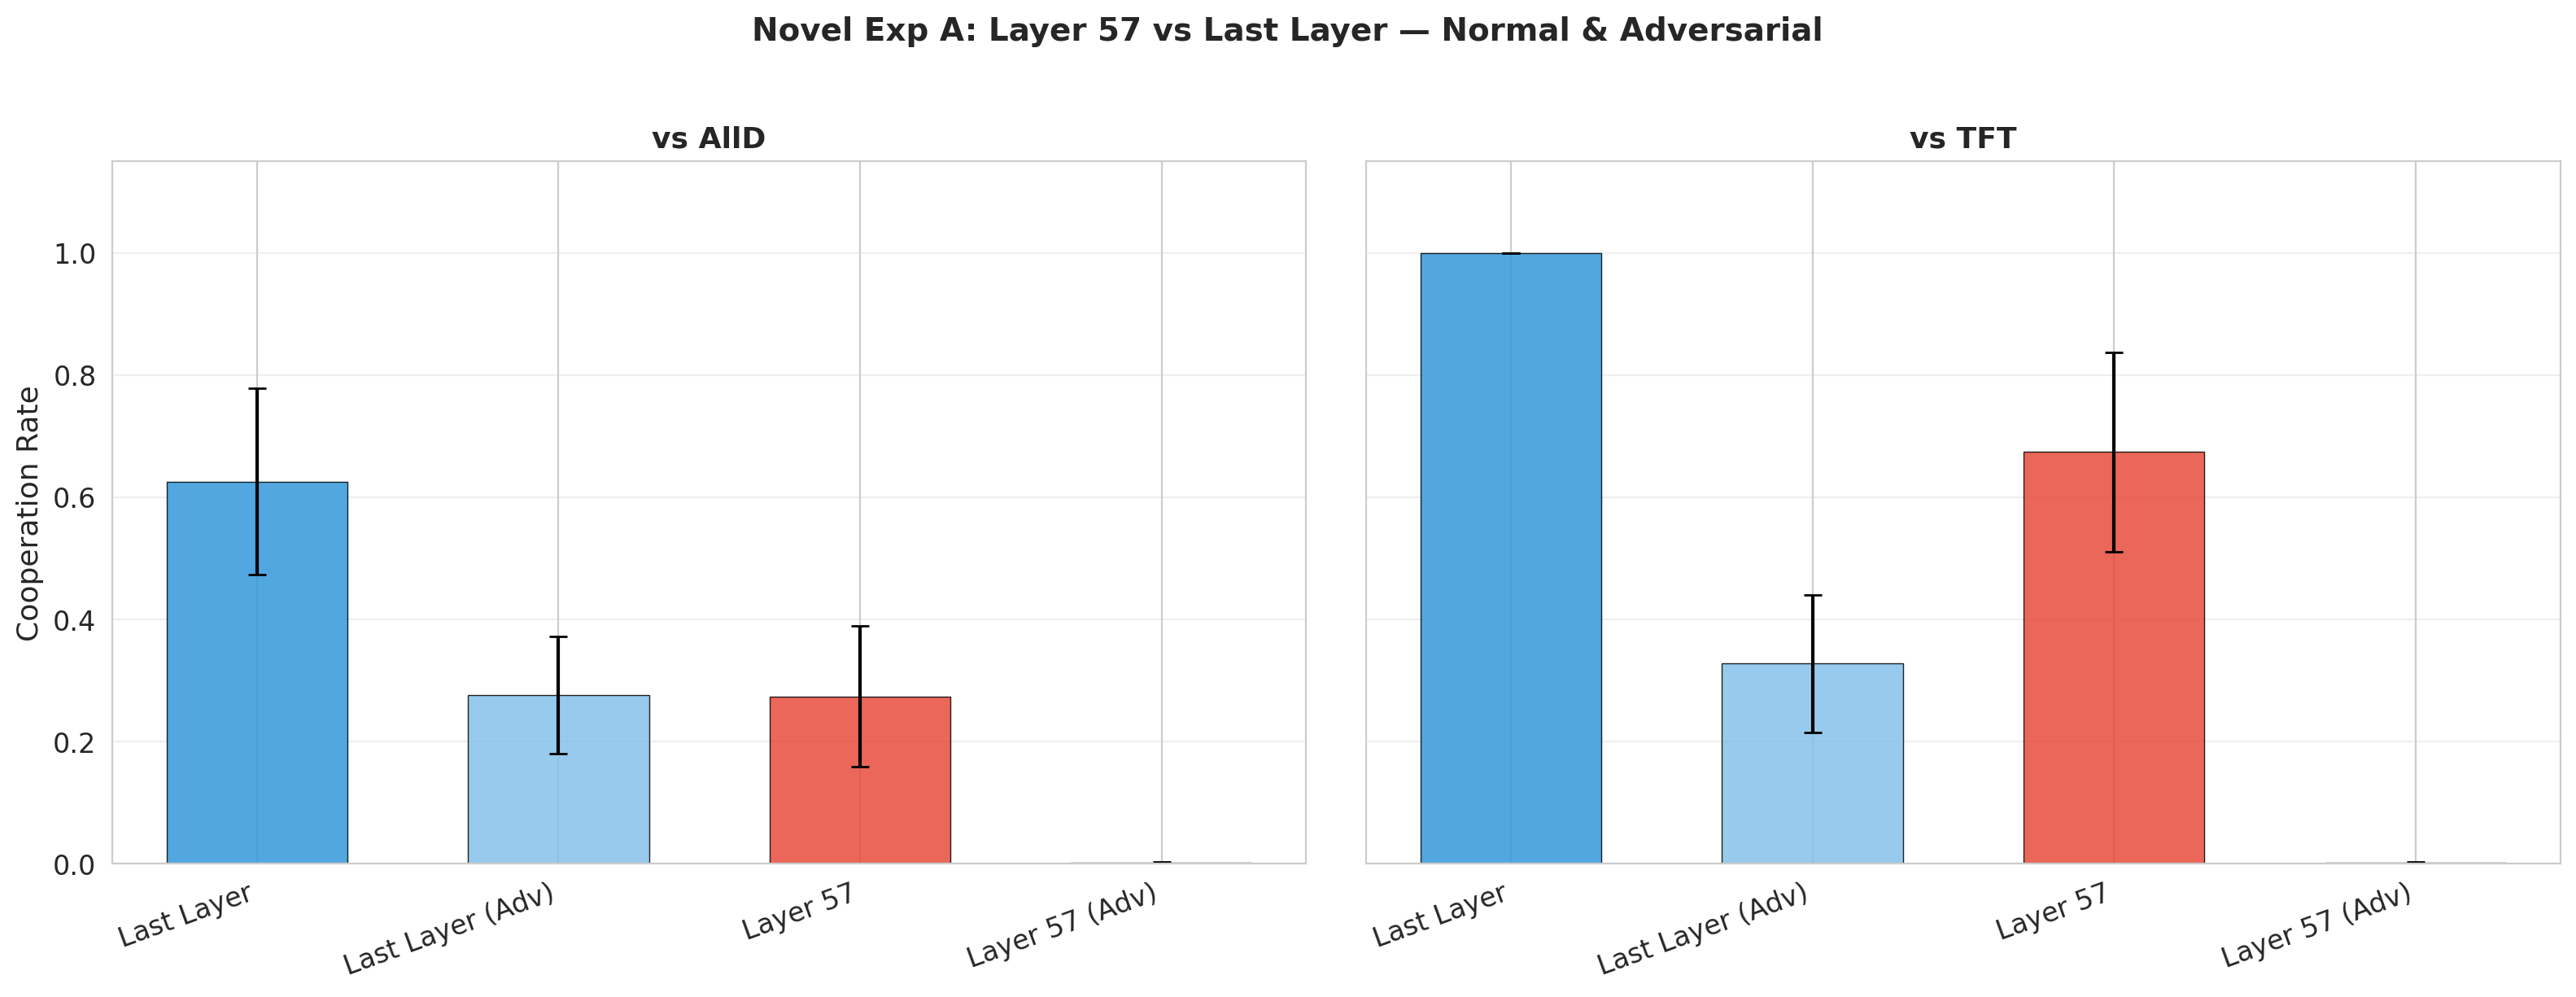
\includegraphics[width=0.85\linewidth]{novel_a_layer_comparison.png}
  \caption{Layer~57 vs.\ last-layer injection under normal and adversarial conditions. Layer~57 is more fragile to adversarial override, consistent with the hypothesis that context integration occurs after the strategic bottleneck.}
  \label{fig:novel_a}
\end{figure}

\subsection{Dynamic vs.\ Static Steering under Adversarial Conditions}
\label{sec:app_dynamic}

Figure~\ref{fig:novel_b} shows the results of Novel Experiment~B, comparing dynamic (latent Tit-for-Tat) steering against static steering and adversarial baselines. Under adversarial prompts, static steering at $\alpha = 0.3$ fails completely ($0\%$ cooperation), matching the adversarial baseline. Dynamic steering---which adapts $\alpha$ based on the opponent's cooperation history---provides partial recovery, achieving $\sim 49\%$ and $\sim 34\%$ mean cooperation under betrayal and dominance adversarial framings respectively. However, the high variance (large error bars) indicates that dynamic adaptation is inconsistent across runs, motivating future work on more robust adaptive mechanisms.

\begin{figure}[h]
  \centering
  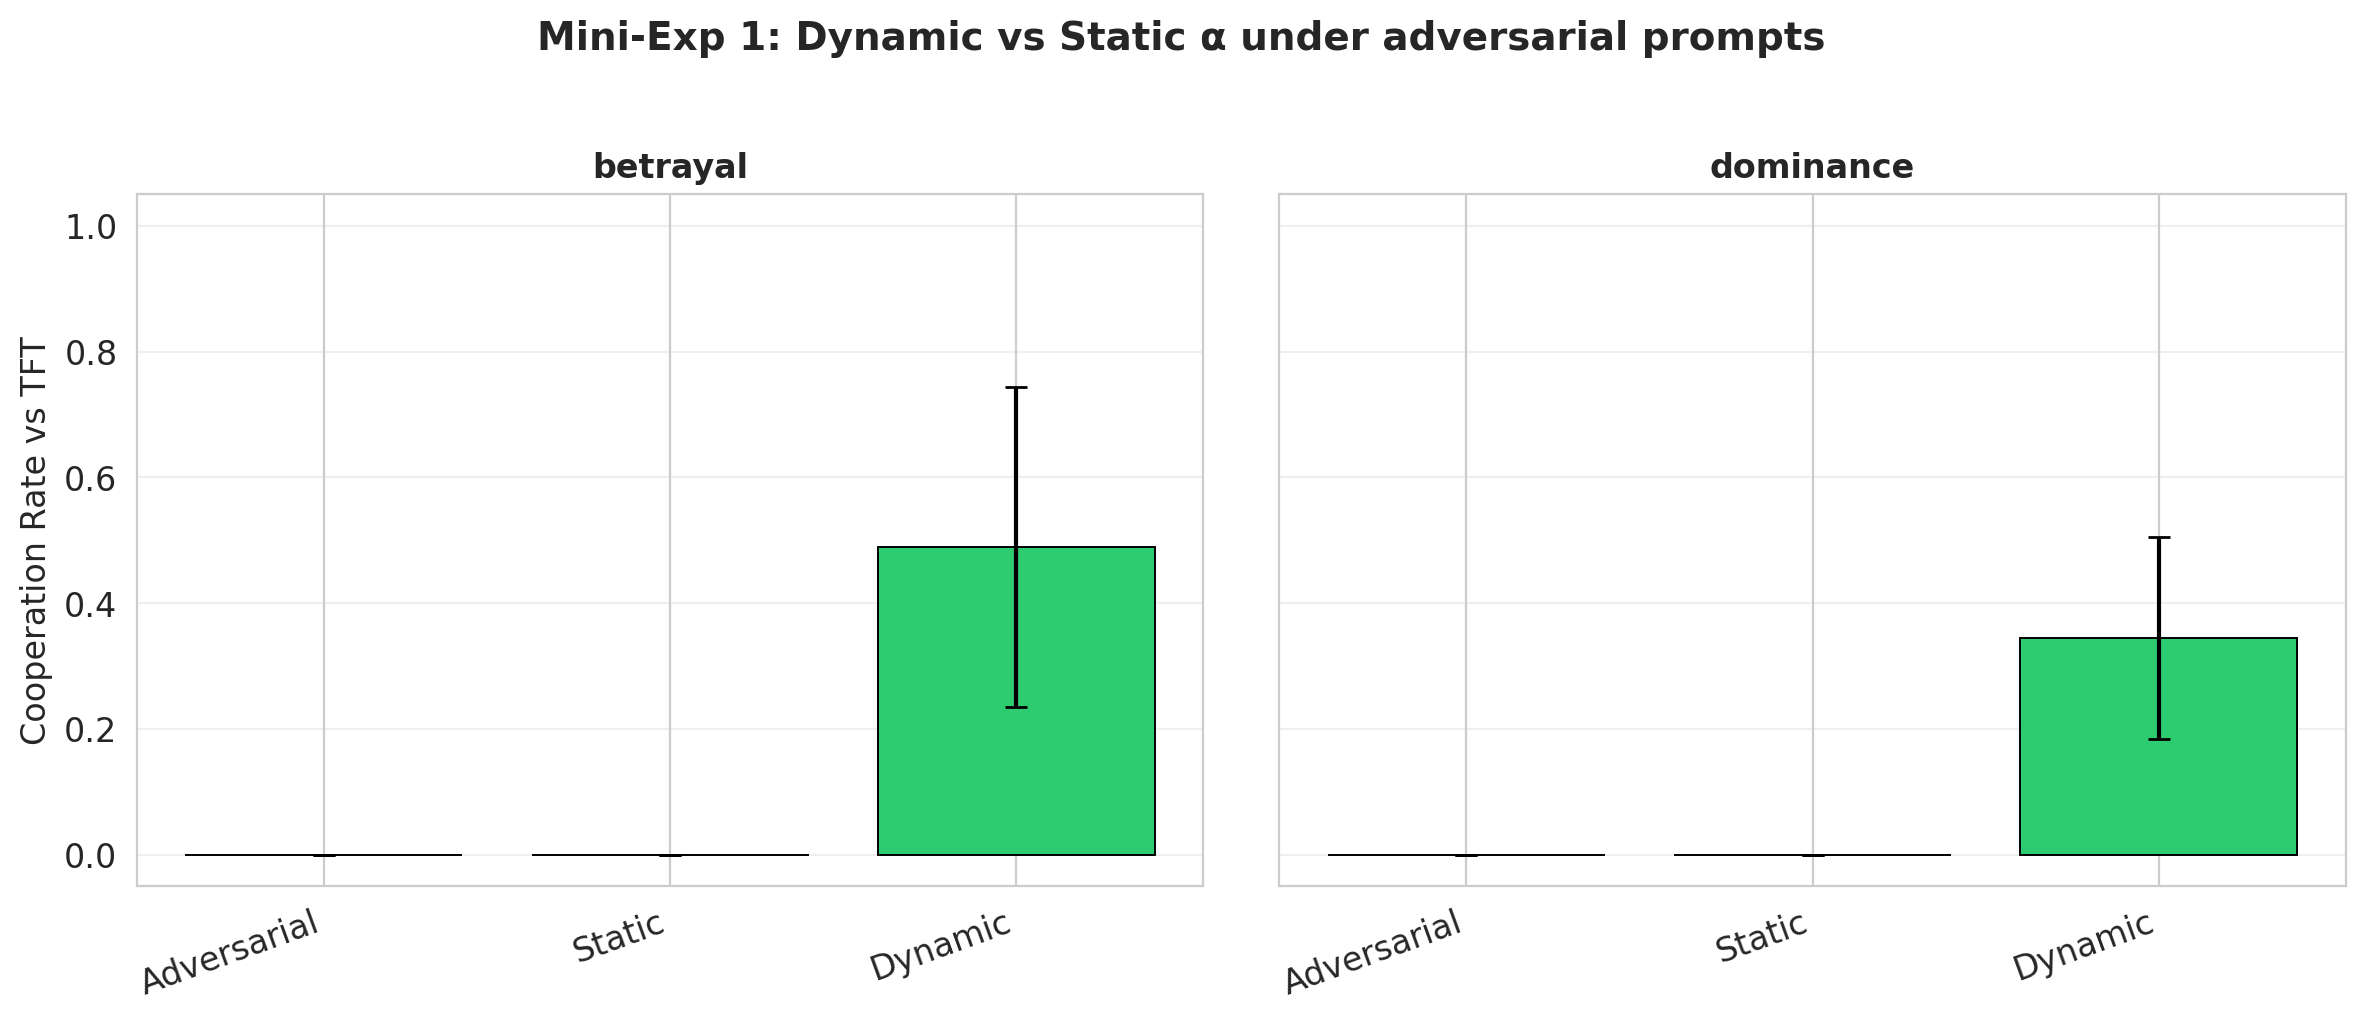
\includegraphics[width=0.85\linewidth]{novel_b_adversarial.png}
  \caption{Dynamic vs.\ static $\alpha$ under adversarial prompts. Dynamic steering provides partial recovery compared to static and adversarial baselines, but with high inter-run variance.}
  \label{fig:novel_b}
\end{figure}

\subsection{Layer $\times$ Alpha Interaction Diagnostic}
\label{sec:app_layer_alpha}

Figure~\ref{fig:layer_alpha} presents a diagnostic heatmap of cooperation rate across 10 layer injection sites and 6 $\alpha$ values against TFT in the Prisoner's Dilemma. The key finding is that \textbf{only Layer~63 at $\alpha = 1.0$} achieves near-complete cooperation ($97\%$), while all other layer--$\alpha$ combinations produce cooperation rates below $38\%$. This demonstrates that steering at individual middle layers (even including the high-FDI Layer~57) is insufficient---the model requires the intervention to propagate through the full residual stream to the final layers for effective behavioral change.

\begin{figure}[h]
  \centering
  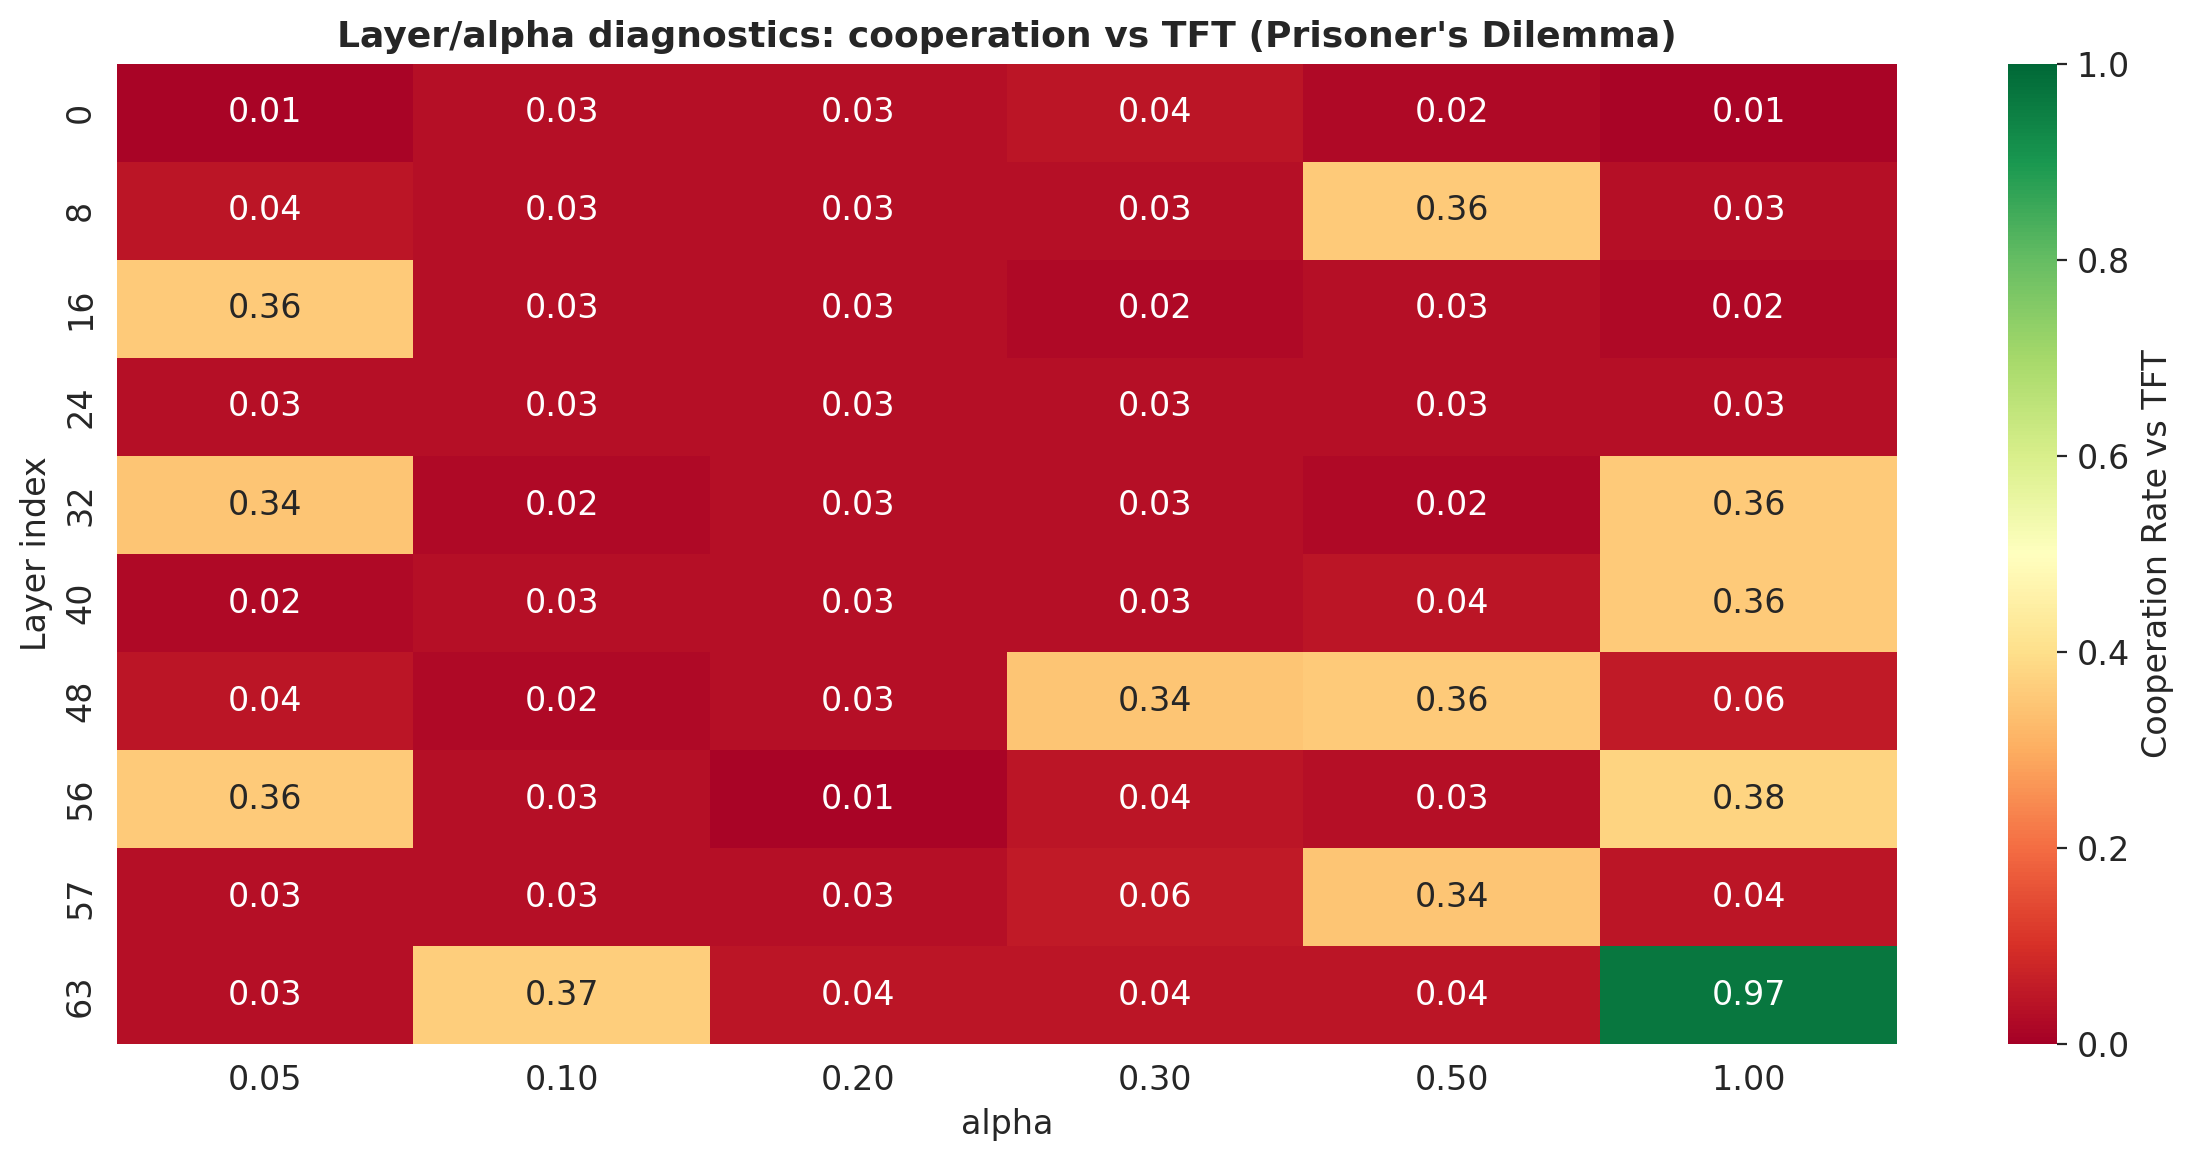
\includegraphics[width=0.85\linewidth]{layer_alpha_diag.png}
  \caption{Layer $\times$ $\alpha$ interaction diagnostic: cooperation rate against TFT across 10 layers and 6 $\alpha$ values. Most cells show near-zero cooperation (red); only the last layer (63) at $\alpha = 1.0$ achieves near-complete cooperation (green).}
  \label{fig:layer_alpha}
\end{figure}


%%%%%%%%%%%%%%%%%%%%%%%%%%%%%%%%%%%%%%%%%%%%%%%%%%%%%%%%%%%%

\newpage
\section*{NeurIPS Paper Checklist}

\begin{enumerate}

\item {\bf Claims}
    \item[] Question: Do the main claims made in the abstract and introduction accurately reflect the paper's contributions and scope?
    \item[] Answer: \answerYes{}
    \item[] Justification: The abstract and introduction explicitly state the scope (game-theoretic evaluation of activation engineering) and four concrete contributions (geometric localization, cross-game transfer, method comparison, and vulnerability analysis), each supported by quantitative results in Section~\ref{sec:exp}.

\item {\bf Limitations}
    \item[] Question: Does the paper discuss the limitations of the work performed by the authors?
    \item[] Answer: \answerYes{}
    \item[] Justification: Section~\ref{sec:exp_robustness} presents the dose-response analysis in detail, and Section~\ref{sec:discussion} extensively discusses limitations including single-model evaluation, the $\alpha$ threshold boundary for adversarial contexts, and ethical dual-use concerns.

\item {\bf Theory Assumptions and Proofs}
    \item[] Question: For each theoretical result, does the paper provide the full set of assumptions and a complete (and correct) proof?
    \item[] Answer: \answerNA{}
    \item[] Justification: The paper is strictly empirical and relies on observational mechanistic interpretability rather than formal mathematical proofs.

\item {\bf Experimental Result Reproducibility}
    \item[] Question: Does the paper fully disclose all the information needed to reproduce the main experimental results?
    \item[] Answer: \answerYes{}
    \item[] Justification: Section~\ref{sec:method} provides the model name, quantization scheme, game environments with payoff matrices, extraction procedure (Eq.~\ref{eq:sv}), intervention algorithm (Algorithm~\ref{alg:steering}), all $\alpha$ values, number of rounds ($T=30$), repetitions ($R=3$), and adversarial prompt templates.

\item {\bf Open access to data and code}
    \item[] Question: Does the paper provide open access to the data and code?
    \item[] Answer: \answerYes{}
    \item[] Justification: Code and raw experimental data (CSV/JSON) are provided in the supplementary material and will be released via an anonymized repository upon acceptance.

\item {\bf Experimental Setting/Details}
    \item[] Question: Does the paper specify all necessary experimental details?
    \item[] Answer: \answerYes{}
    \item[] Justification: All hyperparameters, model configurations, game payoff matrices, opponent strategies, and evaluation protocols are detailed in Section~\ref{sec:method}.

\item {\bf Experiment Statistical Significance}
    \item[] Question: Does the paper report error bars or statistical significance?
    \item[] Answer: \answerYes{}
    \item[] Justification: All results include standard deviations across $R=3$ repetitions. Tables~\ref{tab:cross_game} and \ref{tab:robustness} report mean $\pm$ std.

\item {\bf Experiments Compute Resources}
    \item[] Question: Does the paper provide information on compute resources?
    \item[] Answer: \answerYes{}
    \item[] Justification: Section~\ref{sec:method} discloses the use of a single NVIDIA H100 80GB GPU with 4-bit AWQ quantization.

\item {\bf Code Of Ethics}
    \item[] Question: Does the research conform with the NeurIPS Code of Ethics?
    \item[] Answer: \answerYes{}
    \item[] Justification: The research studies model behavior in simulated game-theoretic environments without deploying agents in real-world settings. Ethical considerations are discussed in Section~\ref{sec:discussion}.

\item {\bf Broader Impacts}
    \item[] Question: Does the paper discuss broader impacts?
    \item[] Answer: \answerYes{}
    \item[] Justification: Section~\ref{sec:discussion} discusses both positive impacts (cooperative alignment) and negative impacts (potential misuse for harmful steering), as well as the dose-response relationship that characterizes the boundary of activation engineering.

\item {\bf Safeguards}
    \item[] Question: Does the paper describe safeguards for responsible release?
    \item[] Answer: \answerNA{}
    \item[] Justification: The paper does not release new pretrained models or risky datasets; it analyzes existing open-weights models using standard game-theoretic environments.

\item {\bf Licenses for existing assets}
    \item[] Question: Are existing assets properly credited?
    \item[] Answer: \answerYes{}
    \item[] Justification: The Qwen2.5 model is properly cited and used in accordance with its open-weights license.

\item {\bf New Assets}
    \item[] Question: Are new assets well-documented?
    \item[] Answer: \answerNA{}
    \item[] Justification: No new large-scale datasets or models are introduced.

\item {\bf Crowdsourcing and Human Subjects}
    \item[] Question: For research with human subjects, are proper protocols followed?
    \item[] Answer: \answerNA{}
    \item[] Justification: The research relies entirely on simulated agent interactions, not human subjects.

\item {\bf IRB Approvals}
    \item[] Question: Were IRB approvals obtained?
    \item[] Answer: \answerNA{}
    \item[] Justification: No human subjects were involved.

\end{enumerate}

\end{document}